\documentclass[12pt]{aghdpl}
% \documentclass[en,11pt]{aghdpl}  % praca w języku angielskim

% Lista wszystkich języków stanowiących języki pozycji bibliograficznych użytych w pracy.
% (Zgodnie z zasadami tworzenia bibliografii każda pozycja powinna zostać utworzona zgodnie z zasadami języka, w którym dana publikacja została napisana.)
\usepackage[english,polish]{babel}

% Użyj polskiego łamania wyrazów (zamiast domyślnego angielskiego).
\usepackage{polski}

\usepackage[utf8]{inputenc}

% dodatkowe pakiety

\usepackage{mathtools}
\usepackage{amsfonts}
\usepackage{amsmath}
\usepackage{amsthm}
\usepackage{array}
\usepackage{tabularx}

\newenvironment{conditions}
{\par\vspace{\abovedisplayskip}\noindent
\tabularx{\textwidth}{>{$}l<{$} @{${}={}$} >{\raggedright\arraybackslash}X}}
{\endtabularx\par\vspace{\belowdisplayskip}}


% --- < bibliografia > ---

\usepackage[
backend=biber,
style=numeric,
sorting=none,
%
% Zastosuj styl wpisu bibliograficznego właściwy językowi publikacji. 
language=autobib,
autolang=other,
% Zapisuj datę dostępu do strony WWW w formacie RRRR-MM-DD.
urldate=iso8601,
% Nie dodawaj numerów stron, na których występuje cytowanie.
backref=false,
% Podawaj ISBN.
isbn=true,
% Nie podawaj URL-i, o ile nie jest to konieczne.
url=false,
%
% Ustawienia związane z polskimi normami dla bibliografii.
maxbibnames=3,
]{biblatex}

\usepackage{csquotes}
% Ponieważ `csquotes` nie posiada polskiego stylu, można skorzystać z mocno zbliżonego stylu chorwackiego.
\DeclareQuoteAlias{croatian}{polish}

\addbibresource{bibliografia.bib}

% Nie wyświetlaj wybranych pól.
%\AtEveryBibitem{\clearfield{note}}


% ------------------------
% --- < listingi > ---

% Użyj czcionki kroju Courier.
\usepackage{courier}

\usepackage{listings}
\lstloadlanguages{TeX}

\lstset{
	literate={ą}{{\k{a}}}1
           {ć}{{\'c}}1
           {ę}{{\k{e}}}1
           {ó}{{\'o}}1
           {ń}{{\'n}}1
           {ł}{{\l{}}}1
           {ś}{{\'s}}1
           {ź}{{\'z}}1
           {ż}{{\.z}}1
           {Ą}{{\k{A}}}1
           {Ć}{{\'C}}1
           {Ę}{{\k{E}}}1
           {Ó}{{\'O}}1
           {Ń}{{\'N}}1
           {Ł}{{\L{}}}1
           {Ś}{{\'S}}1
           {Ź}{{\'Z}}1
           {Ż}{{\.Z}}1,
	basicstyle=\footnotesize\ttfamily,
}

% ------------------------

\AtBeginDocument{
	\renewcommand{\tablename}{Tabela}
	\renewcommand{\figurename}{Rys.}
}

% ------------------------
% --- < tabele > ---

\usepackage{array}
\usepackage{tabularx}
\usepackage{multirow}
\usepackage{booktabs}
\usepackage{makecell}
\usepackage[flushleft]{threeparttable}

% defines the X column to use m (\parbox[c]) instead of p (`parbox[t]`)
\newcolumntype{C}[1]{>{\hsize=#1\hsize\centering\arraybackslash}X}


\newenvironment{abstractpage}
{\cleardoublepage\vspace*{\fill}\thispagestyle{empty} }
{\vfill\cleardoublepage}
\renewenvironment{abstract}[1]
{\bigskip\selectlanguage{#1}%
	\begin{center}\bfseries\abstractname\end{center}}
{\par\bigskip}


%---------------------------------------------------------------------------

\author{Tomasz Kańka}
\shortauthor{T. Kańka}

%\titlePL{Przygotowanie bardzo długiej i pasjonującej pracy dyplomowej w~systemie~\LaTeX}
%\titleEN{Preparation of a very long and fascinating bachelor or master thesis in \LaTeX}

\titlePL{Sprzętowo-programowy system wizyjny do detekcji obiektów zwykorzystaniem termowizji}
\titleEN{Hardware-software vision system for object detection with the use of thermovision.}


\shorttitlePL{Sprzętowo-programowy system wizyjny do detekcji obiektów z wykorzystaniem termowizji} % skrócona wersja tytułu jeśli jest bardzo długi
\shorttitleEN{Hardware-software vision system for object detection with the use of thermovision.}

\thesistype{Praca dyplomowa magisterska}
%\thesistype{Master of Science Thesis}

\supervisor{dr inż. Tomasz Kryjak}
%\supervisor{Marcin Szpyrka PhD, DSc}

\degreeprogramme{Automatyka i Robotyka}
%\degreeprogramme{Computer Science}

\date{2018}

\department{Katedra Automatyki i Robotyki}
%\department{Department of Applied Computer Science}

\faculty{Wydział Elektrotechniki, Automatyki,\protect\\[-1mm] Informatyki i Inżynierii Biomedycznej}
%\faculty{Faculty of Electrical Engineering, Automatics, Computer Science and Biomedical Engineering}

%TODO uzupełnić lub usunąć
\acknowledgements{Serdecznie dziękuję siostrze i ojcu i Ani za użyczenie swojego ciepła.}


\setlength{\cftsecnumwidth}{10mm}

%---------------------------------------------------------------------------
\setcounter{secnumdepth}{4}

\begin{document}

\titlepages

\begin{abstractpage}
	\begin{abstract}{polish}
Dobry system detekcji pieszych znajduje przykładowo zastosowanie w~zaawansowanym wspomaganiu kierowcy. 
W~niniejszej pracy został zaproponowany sprzętowo-programowy system wizyjny bazujący na obrazie multispektralnym. 
Obraz multispektralny jest otrzymywany z połączenia obrazów z~kamery termowizyjnej i wizyjnej. 
Obszar zainteresowania jest wybierany na podstawie klasyfikatora wykorzystującego wzorzec probabilistyczny w~termowizji. 
Następnie wskazany obszar jest ponownie klasyfikowany z~wykorzystaniem HOG i SVM w przestrzeni multispektralnej by potwierdzić obecność przechodnia.
%TODO Gdzie został zaimplementowany i jaka wyjadność dla jakiej rozdzielczości. Ew. jeszcze skuteczność. No i to też w ang.
%TODO Na pewno w mulit ten HOG a nie tylko wizyjnej		
		\textbf{Słowa kluczowe:} 
termowizja, ARM, FPGA, detekcja przechodniów, obraz multispektralny, HOG SVM, wzorzec probabilistyczny
		
	\end{abstract}
	
	\begin{abstract}{english}
A robust pedestrian detection system is crucial in many applications such as advances driver-assistance or video surveillance. 
In this thesis a multispectral image based hardware-software vision system is proposed. 
The multispectral image is obtained by combining outputs of vision and infrared cameras. 
The ROIs (Regions of interest) are selected using a~probabilistic template classifier from infrared image. 
The HOG descriptor and SVM classifier working in multispectral imaging domain is used to confirm that the selected area contains pedestrian.
%TODO uzgonić z wersją PL.
		
		\textbf{Keywords:} 
infrared vision, ARM, FPGA, pedestrian detection, multispectral images, HOG SVM, probabilistic template	
	\end{abstract}
\end{abstractpage}

% Ponowne zdefiniowanie stylu `plain`, aby usunąć numer strony z pierwszej strony spisu treści i poszczególnych rozdziałów.
\fancypagestyle{plain}
{
	% Usuń nagłówek i stopkę
	\fancyhf{}
	% Usuń linie.
	\renewcommand{\headrulewidth}{0pt}
	\renewcommand{\footrulewidth}{0pt}
}

\setcounter{tocdepth}{2}
\tableofcontents
\clearpage

\chapter{Wprowadzenie}

Cyfrowa analiza obrazów znalazła szerokie zastosowanie w~wielu dziedzinach życia.
Dzięki niej możliwe jest automatyczne uzyskanie istotnych dla użytkownika informacji.
Przez ostanie kilkadziesiąt lat opracowano tysiące różnych technik i~algorytmów wyspecjalizowanych do określonych zadań np. leśne fotopułapki do badania zachowań i migracji zwierząt, systemu kontroli jakości i przebiegu procesu przemysłowego, metody kontroli dostępu poprzez rozpoznawanie twarzy m.in. w smartfonach, algorytmu analizy zdjęć satelitarnych ziemi umożliwiające prognozowanie pogody, sterowanie ruchem drogowym na podstawie obrazu z kamer zamontowanych nad skrzyżowaniami, a~także systemy do badania przekroju żołędzia pozwalające określić czy jest on dobrym kandydatem na sadzonkę.

Wzrok ludzki umożliwia rejestrację obrazu w~pewnym zakresie promieniowania elektromagnetycznego zwanego światłem widzialnym.
Dzisiejsza technologia daje możliwość rejestracji poza tym widmem.
Przykładem są kamery termowizyjne, które stają się coraz tańsze i przez to bardziej popularne.
Dostarczają one informację o temperaturze obserwowanych obiektów.
Jest to coraz chętniej wykorzystywane np. w weterynarii do określenia miejsc urazów zwierząt, w~przemyśle do kontroli jakości artykułów spożywczych, w~budownictwie do analizy strat cieplnych w budynkach, w~systemach wspomagania kierowcy do detekcji obiektów w~pobliży drogi, przez ratowników do odnajdywania zasypanych ludzi w~gruzowiskach, straż graniczną do monitorowania granic, przez wojsko do odnajdywania celów i~zagrożeń podczas misji m.in. z wykorzystaniem dronów \cite{gade2014thermal}.
%TODO 2 A tak sobie myślę, czy nie do urazów u ludzi 

Większość systemów wizyjnych służących do detekcji przechodniów jest oparta o~analizę obrazów z~zakresu światła widzialnego bądź podczerwieni.
W przypadku światła widzialnego można uzyskać bardzo dobre wyniki pod warunkiem, że wyszukiwane obiekty są dobrze oświetlone i~wyróżniają się swoim kolorem od tła.
Podczerwień, a~szczególnie termowizja, umożliwia detekcję w~warunkach nocnych i ograniczonej widoczności.
Oba podejścia mają swoje wady i~zalety, które wzajemnie się uzupełniają (np. duże nasłonecznienia powoduje, że tło termiczne staje się dużo wyższe, co utrudnia wyodrębnienie pieszego, natomiast potencjalnie daje idealne warunki do uzyskania dobrej jakości obrazu w~zakresie widzialnym) \cite{lee2015robust}.
Połączenie tych dwóch obrazów daje możliwość uzyskania jeszcze lepszej skuteczności rozpoznawania ludzi.
W pracy \cite{st2007combination} autorzy nazywają ten rozszerzony format jako RGBT (,,Red-Green-Blue-Thermal''), natomiast inna praca jako analizę multispektralną (ang. \textit{Multispectral}) \cite{hwang2015multispectral}, albo po prostu jako połączony obraz z kamery termowizyjnej i~wizyjnej \cite{lee2015robust}.

Skuteczna detekcja obiektów często wymaga dużego zapotrzebowania na zasoby obliczeniowe.
W wielu przypadkach nie da się uzyskać satysfakcjonującej wydajności -- tak by można było uznać system za działający w~czasie rzeczywistym -- wykorzystując jedynie typowy komputer wyposażony w~procesor ogólnego przeznaczenia (nawet najnowszej generacji).
Stosuje się zatem różne metody akceleracji obliczeń.
Jednym z~podejść jest zastosowanie kart graficznych (GPU ang. \textit{Graphics Processing Unit}).
Pozwalają one na duże zrównoleglenie obliczeń, jednak wciąż charakteryzują się znacznym zużyciem energii (choć należy zaznaczyć, że obecnie trwają intensywne prace nad poprawą ich efektywności energetycznej). 
Tworzenie specjalizowanych układów scalonych (ASIC ang. \textit{Application-Specific Integrated Circuit}) daje najlepsze rezultaty w~implementacji systemu wizyjnego, ale ich opracowanie i produkcja wymaga bardzo dużych nakładów finansowych. 

Dobre rozwiązanie stanowią układy rekonfigurowalne, które charakteryzują się podobnymi możliwościami w~realizacji wyspecjalizowanych zadań co układy ASIC, ale nie wymagają tworzenia całkiem nowych układów scalonych. 
Układy FPGA (ang. \textit{Field-Programmable Gate Array}) umożliwiają zrównoleglenie obliczeń i~są szeroko stosowane w systemach wizyjnych.
Szczególnie chętnie są wykorzystywane do realizacji operacji niskiego poziomu, przygotowując wstępnie obraz do dalszej analizy na wysokim poziomie.
Przykłady takich operacji to: filtry konwolucyjne, filtry 2D, podpróbkowanie, wykrywanie krawędzi, obliczanie SAD (ang. \textit{Sum Of Absolute Differences}) z~regionu zainteresowania, obliczanie orientacji krawędzi i~histogramów, obliczanie strumieniowo statystyk (wartość maksymalna, minimalna, średnia), zmiana przestrzeni barw \cite{kisacanin2008embedded}. 
Dodatkową zaletą układów FPGA jest mały pobór mocy, co czyni je niezwykle atrakcyjne dla aplikacji mobilnych -- takich jak drony czy czujniki środowiskowe~\cite{garcia2014survey}.

Układy heterogeniczne łączą w~jednej obudowie dwa układy (zasoby obliczeniowe) o~różanej architekturze i funkcjonalności.
Przykładem takiego połączenia jest Zynq-7000 firmy Xilinx, który integruje w~sobie układ FPGA oraz procesor ARM.
Największą zaletą takiego rozwiązania jest wysoka przepustowość transferu danych między procesorem, a~logiką programowalną, co pozwala na wydajniejszą pracę w przypadku rozdzielenia algorytmu między te dwa układy.
%TODO 2 Tu może jeszcze coś o możliwości podzialu algorymu HW/SW %TT ok

Niniejsza praca stanowi kontynuację i rozwinięcie pracy inżynierskiej autora.

\section{Cel pracy}

Celem pracy była realizacja wbudowanego systemu wizyjnego do detekcji wybranych obiektów (np. ludzi) na podstawie obrazu z kamery termowizyjnej. 
Założono, że jako platforma obliczeniowa zostanie użyty układ heterogeniczny (np. Zynq firmy Xilinx), który umożliwia implementację sprzętowo-programową algorytmów.
W~pierwszym etapie pracy należało dokonać przeglądu i~oceny zrealizowanego w~ramach pracy inżynierskiej algorytmu, a~także przeprowadzić pogłębioną analizę literatury związanej z~tematem. 
Należało przy tym zwrócić szczególną uwagę na systemy detekcji pieszych (wspomaganie kierowcy) oraz systemy dla autonomicznych pojazdów latających (dronów). 
Ponadto należało przeanalizować możliwość wykorzystania kontekstu czasowego tj. informacji zawartej w~sekwencji obrazów. 
Na tej podstawie należało wytypować algorytmy, które zostaną zaimplementowane i przetestowane w aplikacji programowej (Matlab/C++/Python/OpenCV). 
Należało również zgromadzić bazę zdjęć lub sekwencji testowych.

W drugim etapie należało wybrane wspólnie z opiekunem pracy algorytmy zaimplementować w systemie programowo sprzętowym, uruchomić oraz sprawdzić ich skuteczność w różnych scenariuszach testowych.

Oczekiwanym rezultatem pracy był: opis wykorzystania informacji termowizyjnej w~detekcji pieszych (systemy wspomagania kierowcy) oraz detekcji ludzi z wykorzystaniem dronów, implementacja i~analiza kilku podejść (w aplikacji programowej), implementacja sprzętowo-programowo wybranych algorytmów detekcji.

\section{Struktura pracy}

Pracę rozpoczyna wstęp, w którym przestawiono możliwości i~zastosowania kamer termowizyjnych. 
Wskazano również zalety wykorzystania podczerwieni do rozszerzenia spektrum konwencjonalnej kamery wizyjnej -- analizy multispektralnej.
W~rozdziale \ref{cha:multispectral} zostały omówione sposoby uzyskania obrazu multispektralnego. 
Rozdział rozpoczyna się od scharakteryzowania promieniowania podczerwonego oraz metody jego rejestracji. 
Następnie został zaprezentowany model kamery otworkowej oraz transformacja projekcyjna, które stanowią podstawę teoretyczną do prawidłowego połączenia obrazów z dwóch różnych kamer.
W~rozdziale \ref{cha:algoDetPiesz} przedstawiono ogólny przegląd algorytmów służących do detekcji pieszych. 
W~poszczególnych sekcjach zostały omówione kolejne etapy przetwarzania obrazu i~klasyfikacji wraz z~ogólnie stosowanymi rozwiązaniami.%TODO 2 powt. poszczególnych OK
Następnie w~rozdziale \ref{cha:fpga} zostały omówione sposoby zrównoleglenia obliczeń i~możliwość FPGA na przykładzie układu heterogenicznego Zynq-7000 firmy Xilinx.
Kolejny rozdział \ref{cha:przegLiter} zawiera streszczenia kilku wybranych artykułów, które poruszają tematykę związaną z~niniejszą pracą.
W~rozdziale \ref{cha:propSysWiz} przedstawiono koncepcję zaproponowanego rozwiązania wraz ze szczegółami dotyczącymi jego wykonania.
Pracę zakończono podsumowaniem.


\chapter{Multispektralny system wizyjny}
\label{cha:multispectral}

%TODO Kilka zdań o zawratości rozdziału - szczególnie, że jest różnorodna.
%TODO 2 - podtrzymuję powyższe - 2-3 zdania co w rozdziale.
Rozdział rozpoczyna się od charakterystyki promieniowania podczerwonego oraz jego podział na zakresy. Następnie został zaprezentowany sposób rejestracji obrazu termowizyjnego na podstawie kamery Lepton firmy FLIR. Dalej został omówiony dwa sposoby uzyskiwania obrazu poprzez rozdzieleniem wiązki świetlnej na dwa sensory oraz za pomocą układu dwóch kamer równoległych. Następnie został przedstawiony model geometryczny kamery otworkowej oraz sposób kalibracji obrazów zarejestrowanych dwa różnymi kamerami.
 
\section{Podczerwień}

Każde ciało, które ma temperaturę wyższą niż zero absolutne, emituje swoją powierzchnią promieniowanie cieplne. Im wyższa temperatura ciała tym większe natężenie togo promieniowania.
%OK TODO 2 tak Pan to zamotał, że nie wiadomo do czego ,,jej,, się odnosi - temp. czy powierzchni
Dla każdej temperatury danego ciała istnieje charakterystyczna długość fali o~najwyższej wartości mocy promieniowania. 
Wraz z~jej wzrostem, ta częstotliwość przesuwa się w zakres fal widzialnych.
Można to zaobserwować, gdy stal osiąga wysoką temperaturę, co skutkuję emisją światła.
Zależność ta jest opisana prawem Plancka, które opisuję emisję promieniowania elektromagnetycznego przez ciało doskonale czarne.
Ciało doskonale czarne to wyidealizowane ciało fizyczne, które całkowicie pochłania padające na nie promieniowanie oraz emituje promieniowanie ściśle związane z jego temperaturą.
Wykres na rysunku \ref{fig:perfect_black} przedstawia tę zależność.

Mianem podczerwieni określa się promieniowanie elektromagnetyczne w zakresie fali o~długości od 0,75 $\mu m$ do 1000~$\mu m$. Wyróżnia się następujące pasma podczerwieni:
\begin{itemize}
\item Bliska podczerwień (NIR ang. \textit{near infrared}) w~zakresie 0,75 $\mu m$ do 1,4 $\mu m$.
\item Podczerwień fal krótkich (SWIR ang. \textit{short-wawelength infrared}) w~zakresie 1,4$\mu m$ do 3$\mu m$.
\item Podczerwień fal średnich (SWIR ang. \textit{mid-wavelength infrared}) w~zakresie 3$\mu m$ do 8$\mu m$.
\item Podczerwień fal długich (LWIR ang. \textit{long-wavelength infrared}) w~zakresie 8$\mu m$ do 15$\mu m$.
\item Daleka podczerwień (FIR ang. \textit{long-wavelength infrared}) w~zakresie 15$\mu m$ do 1000$\mu m$.
\end{itemize}

Bliska podczerwień znajduje się tuż za zakresem światła widzialnego ludzkim wzrokiem i~jest możliwa do rejestracji przez typowe dla kamer sensory CCD czy CMOS (często z~zastosowaniem dodatkowych oświetlaczy IR). 
Wraz ze wzmacniaczem światła jest również stosowana w~noktowizji.

SWIR i~LWIR występują także pod nazwą termowizji. 
Promieniowanie podczerwone jest częściowo pochłaniane przez atmosferę ziemską. 
Na rysunku \ref{fig:atmosfera_int} przedstawiono tzw. transmisyjność atmosfery. 
W~aparaturze rejestrującej w~podczerwieni wykorzystuje się dwa zakresy, przy których transmisyjność jest największa: 3 -- 5 $\mu m$ oraz 8 -- 14 $\mu m$ \cite{niklaus2007mems}.


\begin{figure}
\centering
\includegraphics[width=0.8\linewidth]{images/Atmosfaerisk_spredning}
\caption[Wykres transmisyjności atmosfery dla promieniowania podczerwonego ]{Wykres transmisyjności atmosfery dla promieniowania podczerwonego \cite{wiki:infrared}.}
\label{fig:perfect_black}
\end{figure}

\begin{figure}
\centering
\includegraphics[width=0.4\linewidth]{images/perfect_black_emi}
\caption[Emisyjność ciała idealnie czarnego]{Emisyjność ciała idealnie czarnego.}
\label{fig:atmosfera_int}
\end{figure}


\section{Kamera termowizyjna}

\subsection{Sensor podczerwieni}

W kamerach do rejestracji obrazu w termowizji są wykorzystywane sensory FPA (ang. \textit{Focal Plane Array} -- płaskie zespoły ogniskujące). 
Najbardziej popularne typy to: InSb (Ind Arsen), InGaAs (Ind Gal Arsen), HgCdTe (Rtęć Kadm Tellur) (w postaci fotodiod; wymagają kriogenicznych warunków pracy) and QWIP (ang. \textit{Quantum well infrared photodetector}). 
Najnowsze technologie wykorzystują niskobudżetowe, niewymagające chłodzenia mikrobolometry. Mikrobolometr jest czujnikiem do pomiaru energii przenoszonej promieniowaniem elektromagnetycznym.
%OK TODO 2 A co to są te mikrobolometry ? Te chemiczne symoble, też może Pan nazwać.

Firma FLIR wykorzystuje tlenek wanadu do budowy mikrobolometrów m.in. w kamerach Lepton. 
Tlenek wanadu cechuje się dużym temperaturowym współczynnikiem rezystancji (TWR) oraz małym szumem 1/f, co zapewnia doskonałą czułość oraz jednolitość. 
W~celu uzyskania obrazu, zespół soczewek skupia promieniowanie z~rejestrowanej sceny na macierz detektorów. 
W~każdym z~detektorów, w~odpowiedzi na padającą na niego wiązkę promieniowania, zmienia się temperatura zawartego w~nim tlenku wanadu. 
Zmiana temperatury wiąże się proporcjonalnie ze zmianą rezystancji. 
Rejestracja sceny polega na odczycie rezystancji każdego detektora poprzez przyłożenia napięcia i~odczyt przepływającego przez nie prądu \cite{flir:lepton}.

%TODO 2 A może znajdzie Pan jakiś rysunek/schemat dla ożywnienia

\subsection{Kamera termowizyjna FLIR Lepton}
\begin{figure}[h]
\centering
\includegraphics[width=0.6\textwidth]{images/Lepton}
\caption{Widok poglądowy na kamerę FLIR Lepton.}
\label{fig:lepton}
\end{figure}

Lepton jest miniaturową kamerą termowizyjną. 
W~pojedynczym układzie został zintegrowany kompletny system składający się soczewki, sensora podczerwieni fal długich (ang. LWIR -- \textit{Long Wave Infrared}) oraz elektroniki sterującej i~przetwarzającej sygnał.
Kamera cechuje się bardzo małymi wymiarami, co czyni ją idealnym rozwiązaniem do zastosowań mobilnych.
Układ ma możliwość domontowania dodatkowej przesłony, która jest wykorzystywana do automatycznej optymalizacji procesu ujednolicania obrazu (kalibracji sensora).
Układ jest prosty do integracji z dowolnym mikrokontrolerem dzięki zastosowaniu standardowych protokołów i interfejsów. Na rysunku /ref{fig:leptonTermalImage} zaprezetowano przykładowy obraz usyskany za pomocą kamery.

Lepton po podłączeniu zasilania od razu uruchamia się w~domyślnym trybie pracy. 
Kamera jest konfigurowalna poprzez CCI (ang. \textit{Camera Control Interface} – interfejs kontroli kamery).
Zapewnia on dostęp do rejestrów zawierających konfigurację \cite{flir:lepton}. 

Parametry kamery:
\begin{itemize}
\item Wymiary: 11,8 x 12,7 x 7,2 mm, 
\item Sensor: niechłodzony mikrobolometr VOx (tlenek wanadu),
\item Rejestrowany zakres: fale długie podczerwieni, 8$\mu m$ do 14$\mu m$,
\item Wielkość piksela: 17 $\mu$m,
\item Rozdzielczość: 80x60 pikseli,
\item Liczba klatek na sekundę: 8,6,  
\item Zakres rejestrowanych temperatur: -10  $^\circ$  C 140  $^\circ$  C (tryb wysokiego wzmocnienia),
\item Korekta niejednorodności matrycy: automatyczna na bazie przepływu optycznego, 
\item Kąt widzenia horyzontalny / diagonalny: 51 $^\circ$  66 $^\circ$,
\item Głębia ostrości: od 10 cm do nieskończoności,
\item Format wyjściowy: do wyboru: 14-bit, 8-bit (z AGC (ang. \textit{automatic gain control} -- automatyczna kontrola wzmocnienia)) 24-bit RGB (z ACG i koloryzacją),
\item Interfejs wideo: VoSPI (Video over Serial Peripherial Interface),
\item Interfejs sterujący: CCI (zbliżony do I2C).
\end{itemize}


\begin{figure}
\centering
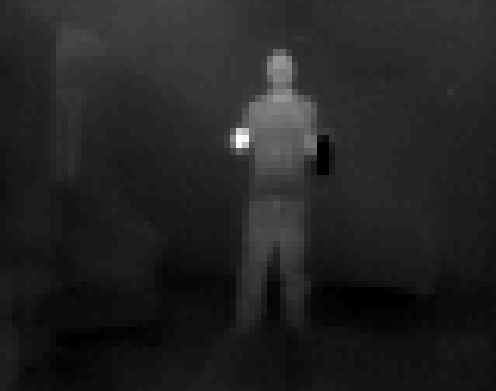
\includegraphics[width=0.5\linewidth]{images/leptonTermalImage.png}
\caption[Obraz człowieka w~termowizji wykonany kamerą Lepton.]{Obraz człowieka w termowizji wykonany kamerą Lepton. W~prawej ręce widać gorący obiekt (kubek herbaty), w~lewej zimny (butelka wody z lodówki).}
\label{fig:leptonTermalImage}
\end{figure}
%OK TODO 2 , ale tradycyjnie - powołanie w tekśie na obraz.



\section{Rejestracja obrazu multispektralnego}

Widmo elektromagnetyczne docierające do kamery składa się fal o~różnych długościach. 
Sensory w~kamerach rejestrują obraz tylko w~pewnym zakresie tego widma, więc aby uzyskać obraz w~wymaganym paśmie należy odfiltrować niepożądane elementy widma, np. kolorowy obraz z kamery wizyjnej jest otrzymywany poprzez zastosowanie trzech filtrów: czerwonego, zielonego i niebieskiego. 
Ponieważ wszystkie trzy kolory mogą być zarejestrowane przez pojedynczą matrycę, filtry są nałożone bezpośrednio na sensor, a~wartość koloru w danym punkcie jest interpolowana z~sąsiadujących ze sobą pikseli (tzw. matryca Bayera). 
W~przypadku, gdy nie jest możliwe zastosowanie jednego sensora do wszystkich pożądanych zakresów, należy rozdzielić wiązkę pomiędzy kilka różnych matryc aparaty, albo wykorzystać równoległy układ kamer. %OK TODO 2 aparaty źle brzmi. Druga sprawa to są takie kamery 3x CMOS, gdzie wiązka jest rozdzialana na trzy czujniki (nie ma tej interpolacji)

W przypadku jednoczesnej rejestracji obrazu wizyjnego i~termicznego większość rozwiązań wykorzystuje układ dwóch równoległych do siebie kamer -- przykład przedstawia rysunek \ref{dual_camera}. 
W tym przypadku została zastosowana kamera termowizyjna FLIR Tao 2 oraz kamera wizyjna Logitech Webcam c600. 

Zazwyczaj obrazy z kamer różnią się, co wynika z ich budowy, różnej rozdzielczości, kąta widzenia oraz zniekształceń soczewkowych.
Do poprawnego odwzorowania tej samej sceny w~obu widmach należy zastosować algorytm mający na celu dopasowanie obu obrazów.
Tworzony jest w~ten sposób nowy obraz, na którym wszystkie piksele łączą informacje o~kolorze i temperaturze.

Pierwszym z~etapów poprawnego dopasowania obrazów jest kalibracja systemu wizyjnego.
Wykonuje się ją z~wykorzystaniem specjalnych plansz, które pozwalają określić położenie pewnych punktów w~przestrzeni w~obu rejestrowanych zakresach promieniowania.
Punkty te pozwalają na obliczenie relacji między obrazami.
Plansze mogą być aktywne (posiadają własne źródło ciepła) albo pasywne (przesłaniają obce źródło ciepła).
W~równoległym układzie kamer występuje również zjawisko paralaksy, które powiększa się wraz ze wzrostem odległości obiektu od punktu kalibracji. Ogranicza to zakres w jakim może działać taki system. %OK TODO 2 to zdanie jest takie na doczepkę. Może napisać co z tego wynika

W~pracy \cite{hwang2015multispectral} autorzy zastosowali zwierciadło półprzezroczyste wykonane z~wafla krzemowego pokrytego cynkiem do rozdzielenia obrazu wizyjnego od termicznego (rysunek \ref{multispectral}). 
Wykorzystując trójosiowy uchwyt, kamery zostały ustawione tak, by ich osie optyczne się pokrywały. 
Następnie obrazy z~obu kamer zostały zrektyfikowane, aby miały tą samą wirtualną ogniskową.

\begin{figure}[h]
\centering
\begin{subfigure}{0.45\textwidth}
\centering
\includegraphics[width=1\textwidth]{images/dual-camera}
\subcaption{\label{dual_camera}}
\end{subfigure}
\begin{subfigure}{0.45\textwidth}
\centering
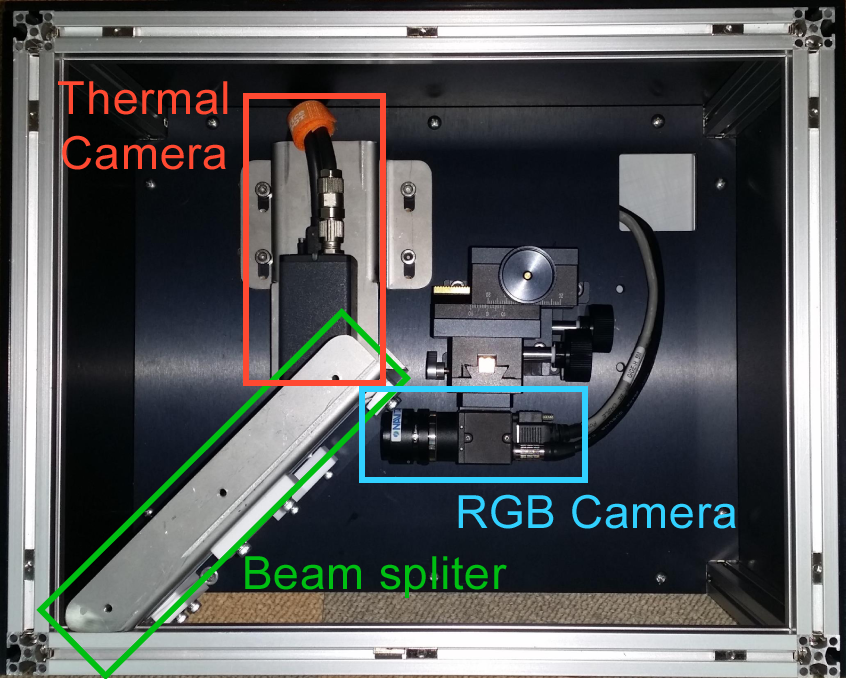
\includegraphics[width=1\textwidth]{images/multispectral}
\subcaption{\label{multispectral}}
\end{subfigure}
\caption{\label{fig:cameras_systems}Sposoby akwizycji obrazów: \protect\subref{dual_camera} dwie kamery równolegle \cite{lee2015robust}, \protect\subref{multispectral} z wykorzystaniem zwierciadła półprzezroczystego \cite{hwang2015multispectral}.}
\end{figure}


\subsection{Model geometryczny}

Do opisu matematycznego systemu wykorzystuje się model kamery otworkowej.
Dzięki niemu można opisać relację między trójwymiarową przestrzenią a~dwuwymiarowym obrazem za pomocą projekcji perspektywicznej. Nie stanowi on najdokładniejszego opisu matematycznego kamery, nie ma w nim uwzględnionych zakłóceń soczewkowych, jednakże zapewnia dobre rezultaty w~większości aplikacji.
Model składa się z~2 zestawów parametrów: zewnętrznych oraz wewnętrznych.
Parametry zewnętrzne definiują lokację kamery względem zewnętrznego układu współrzędnych.
Są reprezentowane przez wektor translacji \(T\) między układem związanym z~kamerą \( \left ( X_{c},Y_{c},Z_{c}\right ) \)
a~zewnętrznym \(\left ( X,Y,Z\right )\).
Drugim parametrem jest macierz rotacji \( R \) (między osiami tych dwóch układów).
Punkt \(P = \left [ X,Y,Z \right ]^T \) będący w~zewnętrznym układzie współrzędnym ma swój odpowiednik w~układzie wewnętrznym, który można określić zależnością:

\begin{equation}
P_{c} = RP+T
\end{equation}

Właściwości optyczne kamery można przedstawić w~postaci macierzy kamery:
\begin{equation}
K = \begin{bmatrix}
f_x & 0 & x_0 \\ 
0 & f_y & y_0\\ 
0 &0 & 1
\end{bmatrix}
\end{equation}
gdzie:
\begin{conditions}
f_{x}, f_{y} & ogniskowa kamery wyrażona w liczbie pikseli, \\
x_{0},y_{0} & współrzędne punktu głównego. 
\end{conditions}

Macierz $K$ określa związek między znormalizowanymi współrzędnymi w~układzie odniesienia kamery danych wzorem \(x_n = \frac{X_c}{Z_c}, y_n = \frac{Y_c}{Z_c}\)  a~odpowiadającym im współrzędnymi punktów na obrazie \(u,v\):

\begin{equation}
\begin{bmatrix}
u \\
v \\
1
\end{bmatrix} = K \begin{bmatrix}
x_n \\
y_n \\
1
\end{bmatrix}
\end{equation}

\subsection{Kalibracja}

Obrazy, które przedstawiają tę samą scenę, ale zostały wykonane dwoma różnymi kamerami w~innych położeniach różnią się. 
Na rysunku \ref{fig:oneSceaneTwoCameras} czarna szachownica jest uchwycona przez dwie kamery ustawione w~punktach $C_A$ (na wprost obiektu) oraz $C_B$ (po skosie i~lekko obrócona).

\begin{figure}
\centering
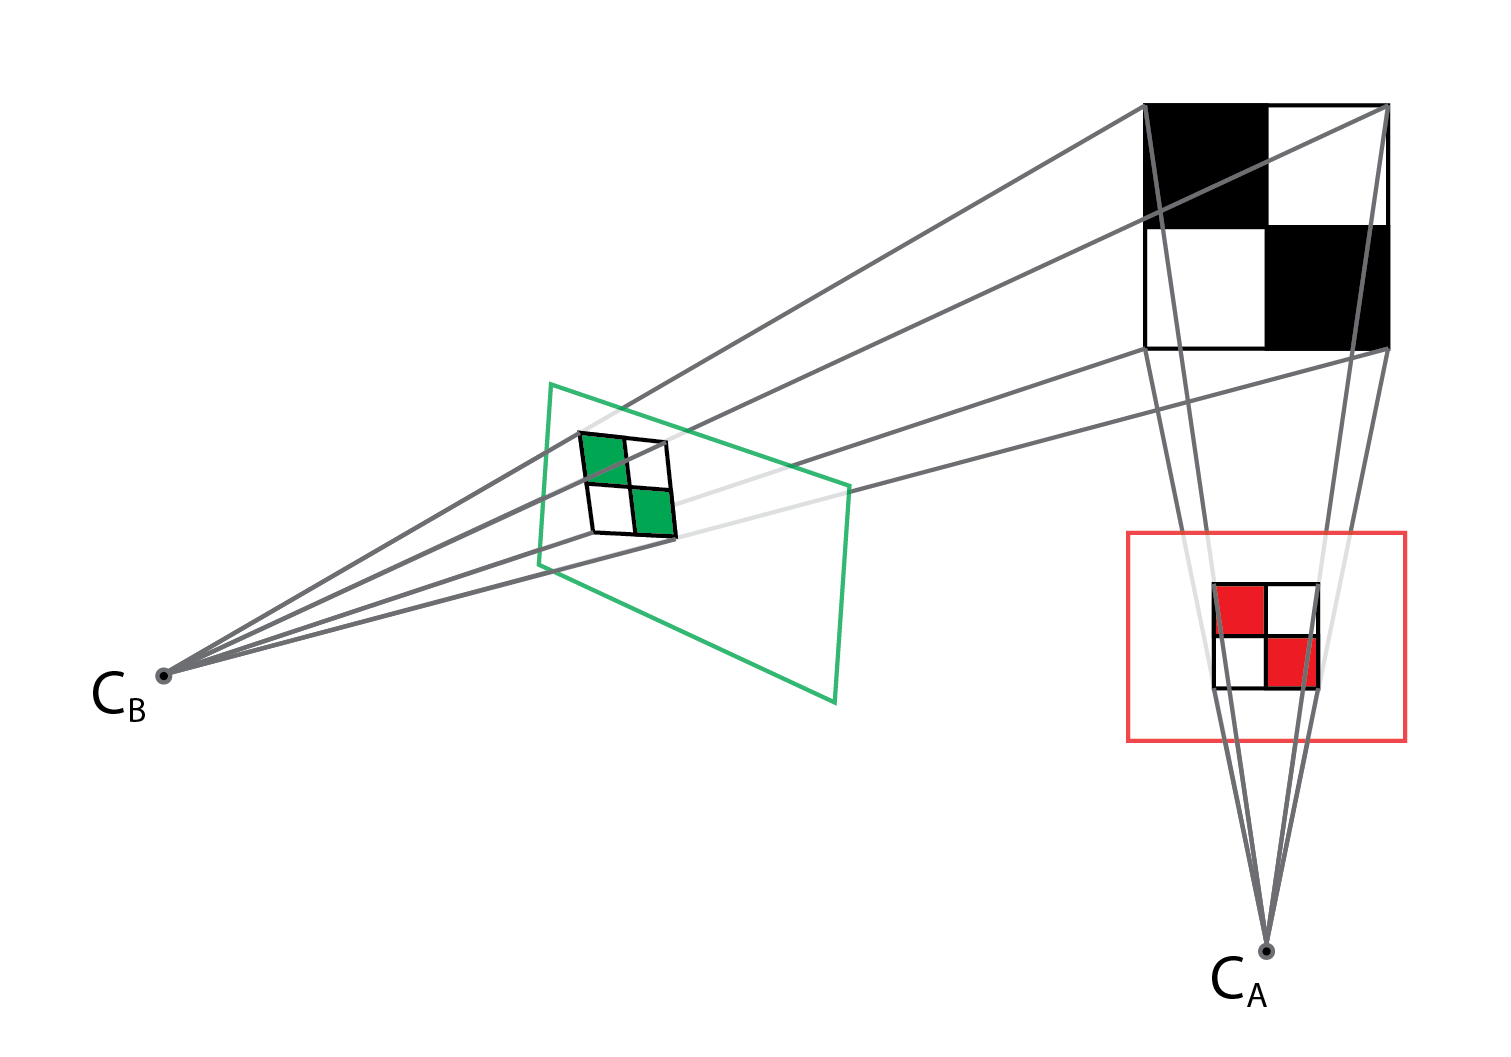
\includegraphics[width=0.6\linewidth]{images/oneSceaneTwoCameras}
\caption[Dwie kamery rejestrujące jeden obiekt. ]{Dwie kamery rejestrujące jeden obiekt.}
\label{fig:oneSceaneTwoCameras}
\end{figure}

Aby dopasować te dwa obrazy, tak by szachownice były ujęte tak samo (tj. w~tym samym miejscu na obrazie), należy na jednym z~nich przeprowadzić transformację projekcyjną. 
Jest to przekształcenie pomiędzy dwoma płaszczyznami, które wykorzystuje model geometryczny kamery. 
Wymaga to uprzedniego wyznaczenia macierzy transformacji $A$ na podstawie co najmniej 4 punktów kalibracyjnych.

\begin{figure}[h]
\centering
\begin{subfigure}{0.30\textwidth}
\centering
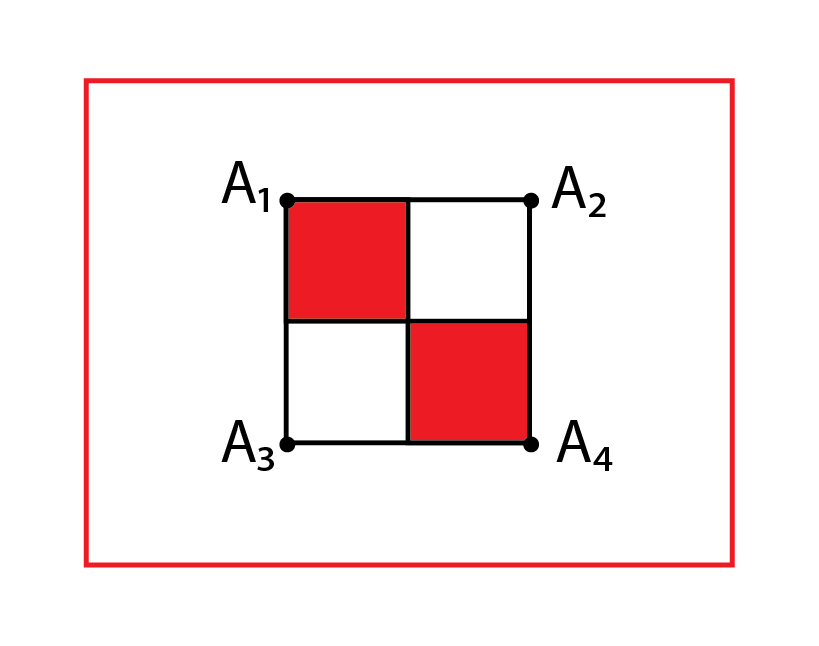
\includegraphics[width=1\textwidth]{images/camAimage}
\subcaption{\label{fig:camAimage}}
\end{subfigure}
\begin{subfigure}{0.30\textwidth}
\centering
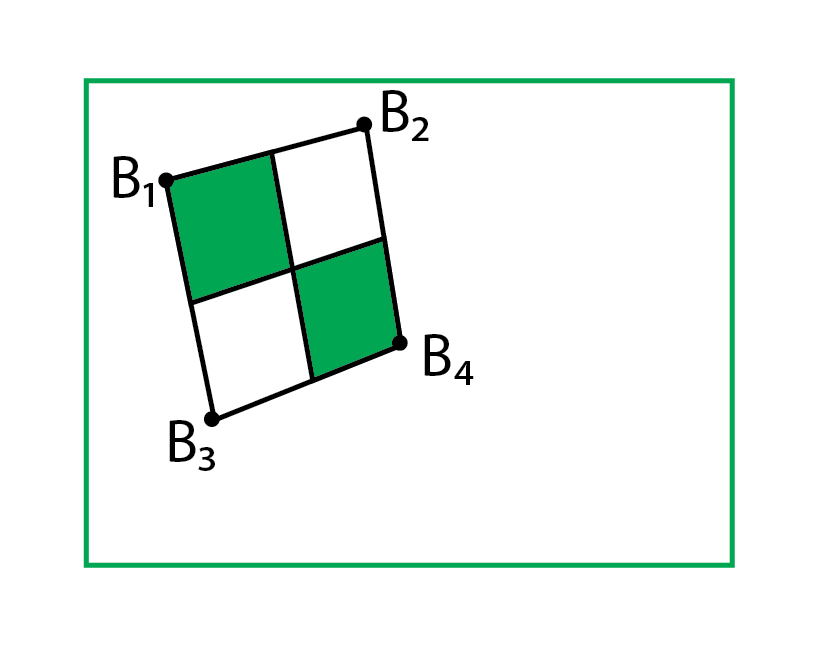
\includegraphics[width=1\textwidth]{images/camBimage}
\subcaption{\label{fig:camBimage}}
\end{subfigure}
\caption{\label{fig:camImages}Zarejestrowane obrazy: \protect\subref{fig:camAimage} przez kamerę $C_A$, \protect\subref{fig:camBimage} przez kamerę $C_B$. Punkty $A$ i $B$ są punktami kalibracyjnymi.}
\end{figure}

Na rysunkach \ref{fig:camAimage} i~\ref{fig:camBimage} punkty $A_1$ do $A_4$, będące czterema rogami zarejestrowanej szachownicy przez kamerę $C_A$, odpowiadają punktom $B_1$ do $B_4$, będącymi tymi samymi czterema rogami zarejestrowanymi kamerą $C_B$. Macierz transformacji $A$ można obliczyć rozwiązując równanie \eqref{transformMatrix}:
\begin{equation}
\label{transformMatrix}
A = \begin{bmatrix}
a & b & c\\ 
d & e & f\\ 
g & h & 1
\end{bmatrix}
\end{equation}

\begin{equation}
\begin{bmatrix}
u_1\\ 
u_2\\ 
u_3\\ 
u_4\\
...\\ 
u_n\\ 
v_1\\ 
v_2\\ 
v_3\\ 
v_4\\ 
...\\ 
v_n 

\end{bmatrix}
=
\begin{bmatrix}
x_1 & y_1 & 1 & 0 & 0 & 0 & -u_1x_1 & -u_1y_1\\ 
x_2 & y_2 & 1 & 0 & 0 & 0 & -u_2x_2 & -u_2y_2\\ 
x_3 & y_3 & 1 & 0 & 0 & 0 & -u_3x_3 & -u_3y_3\\ 
x_4 & y_4 & 1 & 0 & 0 & 0 & -u_4x_4 & -u_4y_4\\ 
...\\ 
x_n & x_n & 1 & 0 & 0 & 0 & -u_nx_n & -u_ny_n\\ 
0 & 0 & 0 & x_1 & y_1 & 1 & -v_1x_1 & -v_1y_1\\ 
0 & 0 & 0 & x_2 & y_2 & 1 & -v_2x_2 & -v_2y_2\\  
0 & 0 & 0 & x_3 & y_3 & 1 & -v_3x_3 & -v_3y_3\\ 
0 & 0 & 0 & x_4 & y_4 & 1 & -v_4x_4 & -v_4y_4\\ 
...\\ 
0 & 0 & 0 & x_n & y_n & 1 & -v_nx_n & -v_ny_n
\end{bmatrix}
\begin{bmatrix}
a \\
b\\
c\\
d \\
e\\
f\\
g\\
h
\end{bmatrix}
\end{equation}

\begin{conditions}
u_{n},v_{n} & współrzędne punktu kalibracji $n$, na obrazie bazowym\\
x_{n},y_{n} & współrzędne punktu kalibracji $n$, na obrazie dopasowywanym 
\end{conditions}

Transformację projekcyjną można zinterpretować jako rzutowanie płaszczyzny, co obrazuję rysunek \ref{fig:projection}. 
Wynikiem transformacji (a~zarazem rzutowania) jest obraz dopasowany do obrazu bazowego (\ref{fig:projectionImage})


\begin{figure}
\centering
\begin{subfigure}{0.47\textwidth}
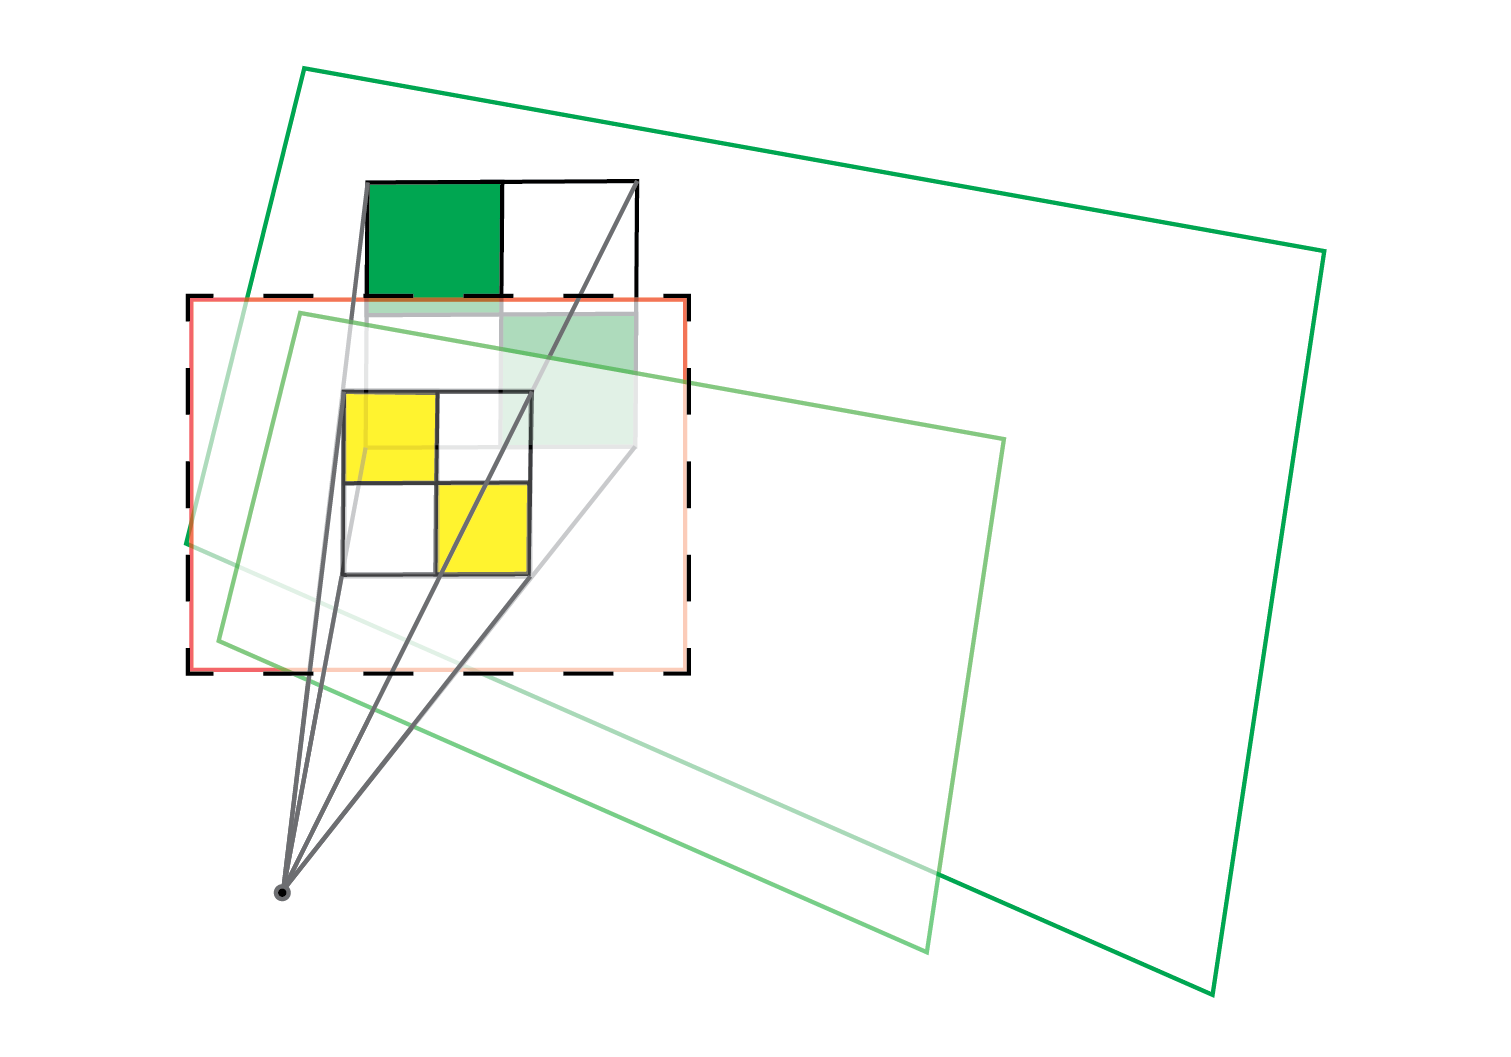
\includegraphics[width=0.9\linewidth]{images/projection}
\caption[Interpretacja transformacji projekcyjnej: rzutowanie płaszczyzny. ]{Interpretacja transformacji projekcyjnej: rzutowanie płaszczyzny.}
\label{fig:projection}
\end{subfigure}
\begin{subfigure}{0.47\textwidth}
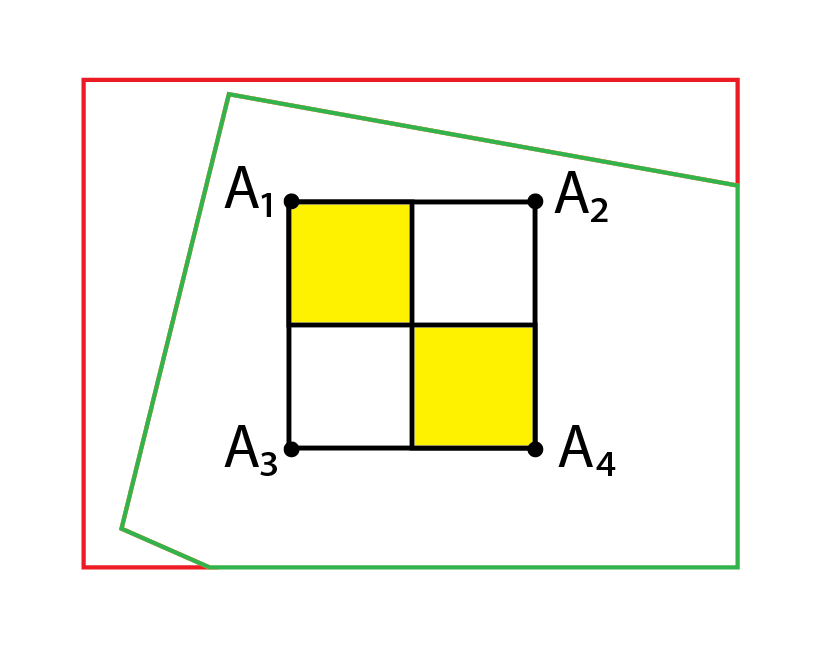
\includegraphics[width=0.9\linewidth]{images/projectionImage}
\caption[Wynik transformacji. ]{Wynik transformacji.}
\label{fig:projectionImage}
\end{subfigure}
\caption[Transformacja projekcyjna ]{Transformacja projekcyjna.}
\end{figure}

\chapter{Algorytmy detekcji pieszych}
\label{cha:algoDetPiesz}

W~cyfrowej analizie obrazu detekcja pieszych jest jedną z~najbardziej aktywnie rozwijanych dziedzin.
W~ciągu kilkudziesięciu lat powstało ponad tysiąc artykułów poruszających to zagadnienie \cite{zhang2015filtered}, w~których zaproponowano wiele różnych metod.
Większość z~nich opiera się na analizie obrazu tylko w~jednym spektrum: widzialnym albo podczerwieni.
Praca \cite{hwang2015multispectral} pokazała, iż połączenie obu obrazów może dać lepsze wyniki.
Podobnie w~artykule \cite{gonzalez2016pedestrian} wykazano, że analiza multispektralna jest skuteczniejsza w~dzień niż w~nocy (o~około 5\% AMR (ang. \textit{Avrange Miss Rate}).
W~artykule \cite{benenson2014ten} autorzy podsumowują osiągnięcia w~dziedzinie detekcji pieszych w latach 2004 -- 2014.
Wyróżniono ponad 40 różnych podejść do problemu.
Eksperymenty w~artykule są oparte o~bazę danych Caltech-USA, która zawiera obrazy w~kolorze.
Jednym z wniosków jest to, że przez ostanie dziesięć lat największy postęp został osiągnięty głównie dzięki dopracowaniu cech, które są wyodrębniane z obrazu, niż ulepszanie klasyfikatora.
Dodatkowo autorzy połączyli cechy dające najlepsze wyniki i~stworzyli własną metodę, która pozwoliła poprawić o~ok 12\% AMR względem najlepszej badanej wcześniej metody.

Coraz większą popularnością cieszą się rozwiązania oparte o głębokie sieci neuronowe  (DNN ang. \textit{Deep Neural Networks}). W artykule \cite{du2017fused} został zaprezentowany system wykrywania pieszych operaty na fuzji kilkunastu dobrze wyuczonych sieci neuronowych, dając jeden z lepszych wyników detekcji z wykorzystaniem bazy Caltech-USA. 
%ok TODO a coś o głębokich sieciach ? Jakoś pominął Pan ten temat.
%ok TODO 2 jw. ? chociaż jeden przykład - bo to jest teraz na topie....

Dla typowego algorytmu detekcji pieszych można wyróżnić trzy podstawowe etapy:

\section{Ustalenie regionu zainteresowania}

Jest to obszar zwany ROI (ang. \textit{Region Of Interest}), w~którym potencjalnie mogą znajdować się piesi.
Wiele podejść uznaje cały obraz jako ROI i~stosuje okno przesuwne, sprawdzając każdy możliwy fragment obrazu.
Jeżeli scena jest rejestrowana przez nieruchomą kamerę, ROI można określić poprzez różnicę między zapamiętanym tłem a~aktualnym obrazem (tzn. modelowanie i~odejmowanie tła). 
Analiza przepływu optycznego również pozwala na wyodrębnienie obszaru, w~których obserwowany jest ruch inny niż na pozostałej części sceny. 
Inną metodą jest zastosowanie słabszego, bardziej ogólnego, ale mniej wymagającego obliczeniowo  klasyfikatora.
Wyodrębnienie ROI jest bardzo istotne w~przypadku pracy w~czasie rzeczywistym, ze względu na ograniczony maksymalny czas analizy pojedynczego obrazu.

\section{Wyodrębnienie cech}

Do najbardziej popularnych cech można zaliczyć:

\begin{enumerate}
\item Histogramy zorientowanych gradientów (HOG ang. \textit{Histogram of Oriented Gradients }).
Algorytm został zaproponowany przez N.Dalala i B. Triggsa w~pracy \cite{dalal2005histograms} i~stał się jedną z~najbardziej popularnych metod w~dziedzinie detekcji ludzi. 
Jest cały czas rozwijany i~modyfikowany w~wielu pracach naukowych.
W pierwszej kolejności zostają obliczone gradienty dla obrazu, za pomocą dwóch masek kierunkowych [-1 0 1] i [-1 0 1]$^T$. Gradienty mogą być ze znakiem lub bez. Na rysunku \ref{fig:hog} przedstawiono przykład uzyskiwania gradientów. Następnie tworzone są histogramy orientacji na podstawie gradientów uzyskanych z pkt. 1. Histogram ma z~góry zadaną liczbę przedziałów i zawiera dane z komórki (ang. \textit{cell}) o określonej wielkości (np. kwadrat 6x6). Wagi orientacji poszczególnych pikseli wynikają z wartości wypadkowej gradientu. Na rysunku \ref{fig:hog2} zaprezentowano przykładowe histogramy.
Komórki łączone są w bloki, w obrębie których następuje normalizacja. Ma ona na celu wyrównanie kontrastów pomiędzy sąsiadującymi blokami komórek. Bloki mają z góry ustalony rozmiar i nakładają się na siebie. Połączenie wszystkich histogramów we wszystkich blokach w jeden wektor cech.

\begin{figure}
\centering
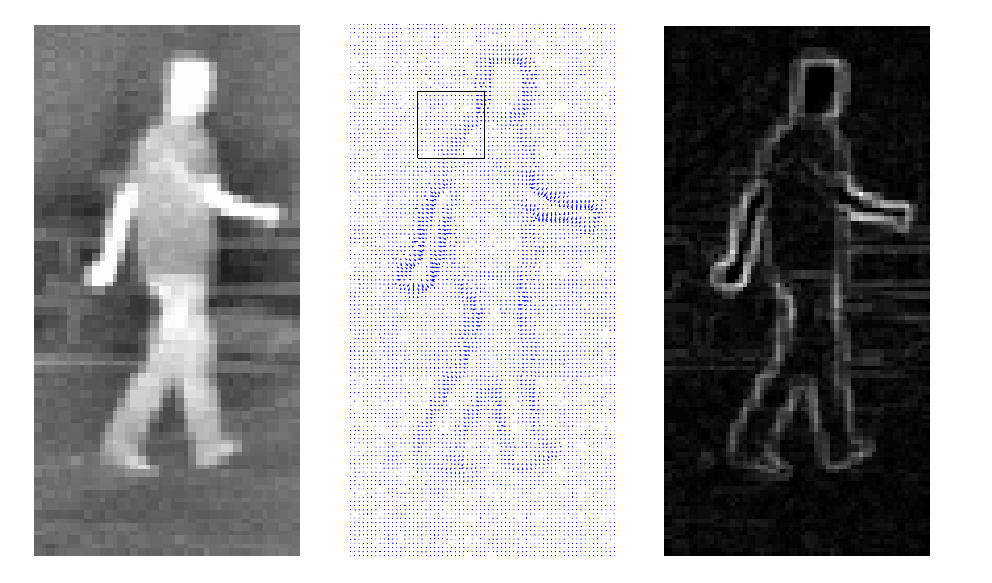
\includegraphics[width=0.5\linewidth]{images/hog}
\caption[Obliczanie gradientów dla obrazu.]{Obliczanie gradientów dla obrazu. Po lewej oryginalny obraz, pośrodku kierunki gradientów, po prawej wartości modułów \cite{suard2006pedestrian}.}
\label{fig:hog}
\end{figure}

\begin{figure}
\centering
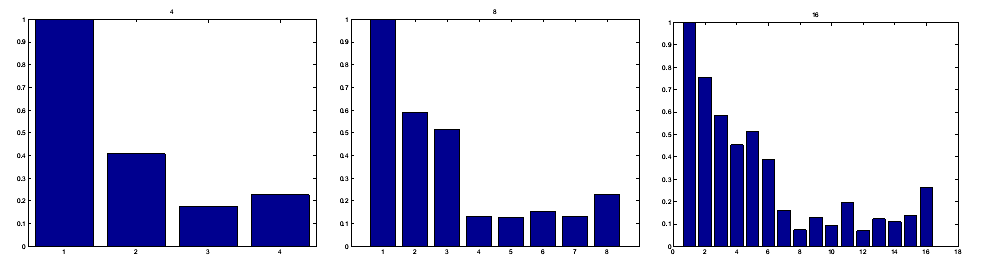
\includegraphics[width=0.7\linewidth]{images/hog2}
\caption[Przykładowe histogramy]{Przykłady histogramów o różnej ilości przedziałów \cite{suard2006pedestrian}.}
\label{fig:hog2}
\end{figure}

%TT w dalszym rozdziale jest to szczegółowo opsane.
%TODO 2 Skoro tak to proszę dać więcej szczegółów 

\item Lokalne wzorce binarne LBP (ang. \textit{Local Binary Paterns}).
Oryginalnie deskryptory te zostały zaproponowane  do opisu tekstur \cite{ojala2002multiresolution}. %OK TODO \cite też coś ojala - 2 tego Pan nie zrobił.
Analizowany obraz zostaje podzielony na bloki.
Następnie, do każdego piksela w~bloku zostaje przypisany wzorzec binarny na podstawie wartości pikseli w~jego sąsiedztwie.
Jeżeli wartość sąsiadującego piksela jest większa od centralnego, to przyjmuje on wartość~1. 
W~ten sposób do każdego piksela przypisywany jest wzorzec binarny (np. 1100110). %OK TODO 2 7 bitów.. raczej 8
Następnie zostaje obliczony histogram wzorców dla każdego bloku.
Histogramy z wszystkich bloków wchodzących w~skład obrazu (okna detekcji) tworzą wektor cech.

\item Falki Haara.
Określają różnicę w~kontraście między dwoma przylegającymi prostokątnymi obszarami. 
W~oryginalnej pracy P.Viola i M.Jones z~2001 \cite{viola2001rapid} autorzy rozważali 3 rodzaje cech: 
\begin{itemize}
	\item dwa obszary mające ten sam rozmiar i~kształt oraz przylegające do siebie horyzontalnie bądź wertykalnie, gdzie cechę stanowi różnica sumy pikseli zawartych w~każdym z regionów ( Układ A i B na rysunku \ref{fig:haar}), 
	\item obszar składający się z 3 prostokątów przylegających do siebie, gdzie od sumy środkowego elementu jest odejmowana suma dwóch zewnętrznych (układ~C),
	\item układ 4 prostokątów, gdzie suma jest różnicą między obszarami po przekątnej (układ~D). %OK TODO 2 niejasne...
\end{itemize}

\begin{figure}
\centering
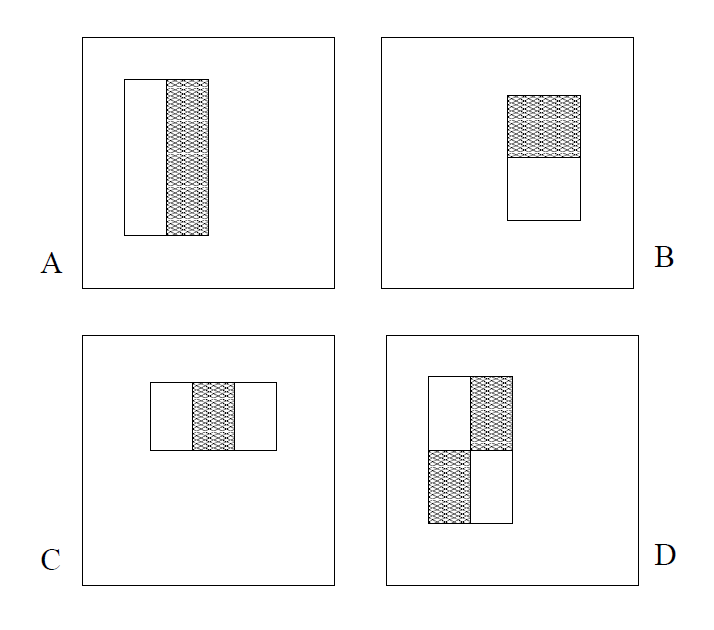
\includegraphics[width=0.4\linewidth]{images/haar}
\caption[Falki Harrra.]{Przykładowe prostokąty służące do określenia cech. Od sumy pikseli zawartych w~białym prostokącie zostaje odjęta suma pikseli w~szarym. \cite{viola2001rapid}.}
\label{fig:haar}
\end{figure}
%OK TODO 2 obrazek by bardzo pomógł
Cechy są łatwe do skalowania i~nie wymagają dużych nakładów obliczeniowych. W celu szybkiego obliczania tych cech stosuje się tzw. \textit{intergral image}. Dla każdego puntu o~współrzędnych x,y zostaje obliczona suma wartości pikseli znajdujących się na lewo i~nad pozycją~x,y. Dzięki temu, aby obliczyć sumę pikseli w~danym kwadracie wystarczą jedynie cztery punkty referencyjne. Na przykład, by obliczyć sumę pikseli w~prostokącie D na rysunku \ref{fig:integralImage} wystarczy rozwiązać równanie $D = 4 + 1 -(2 + 3)$.

\begin{figure}
\centering
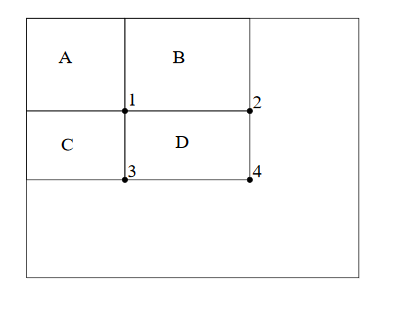
\includegraphics[width=0.4\linewidth]{images/integralImage}
\caption[IntegralImage.]{Obliczanie sumy pikseli za pomocą \textit{integral image}.  \cite{viola2001rapid}.}
\label{fig:integralImage}
\end{figure}
%OK TODO 2 można Pan dodać, że ich do ich obliczania można wykorzystać tzw. intergral image.

\item Kolor. 
W~analizie obrazów wykorzystuje różne przestrzenie barw np. RGB, HSV oraz LUV. 
Głównie wtedy, gdy kolor wykrywanego obiektu jest kluczowy (np. znaki drogowe, światła na skrzyżowaniu). 
Jako cechę można go wykorzystać w~kilku formach. 
Momenty koloru (ang. \textit{Color Moments}) jest to średnia, wariancja i~odchylenie standardowe występowania danego koloru na obrazie. 
Histogram określa częstość występowania danego koloru, a~wektor koherencji koloru (CCV ang. \textit{Color Coherence Vectors}) określa w~jakim stopniu piksele danego koloru są częścią obszaru o~podobnym kolorze (np. obraz zielonej łąki na którym pasie się jedna fioletowa krowa. Kolor zielony na obrazie byłby rozłożony równomiernie natomiast fioletowy byłby skupiony w~pojedynczym rejonie koherencji -- krowy) \cite{kodituwakku2004comparison}.

\end{enumerate}

\section{Klasyfikator}

Otrzymany wektor cech jest następnie poddany klasyfikacji, której wynik decyduje czy obraz zawiera człowieka.
W pracy \cite{benenson2014ten} autorzy wyróżnili 3 dominujące rodziny metod:

\begin{enumerate}
\item Rodzina DPM (ang. \textit{Deformable Part Model})
%
Technika zakłada, że obiekty mogą być zamodelowane poprzez części ułożone w~deformowanych konfiguracjach. 
Model składa się z~głównego, globalnego filtra, który stanowi punkt odniesienia dla pozostałych części. 
Każda część zawiera swój własny filtr wraz z~zestawem dozwolonych pozycji względem okna detekcyjnego oraz koszt deformacji dla każdej z tych pozycji. 
Suma wyniku uzyskanego z~filtra głównego wraz z~jego częściami stanowi o~wyniku detekcji \cite{felzenszwalb2008discriminatively}.

\item Deep networks.
%OK TODO 2 1. Musi Pan wraznie zaznaczyć, że to jest nieco odrebne, w sensie ze to jest ekstrakca + klasyfikacja.
%OK TODO 2 2. Jakiś rysunek by też pomógł.

\begin{figure}
\centering
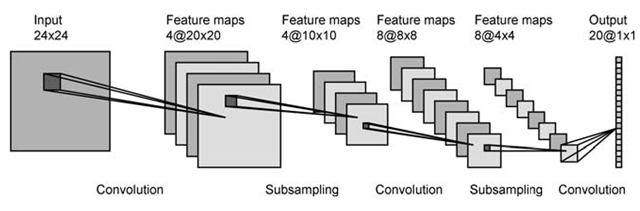
\includegraphics[width=0.8\linewidth]{images/DNN}
\caption[IntegralImage.]{Schemat przykładowej sieci konwolucyjnej.}
\label{fig:DNN}
\end{figure}

Głębokie sieci neuronowe posiadają kilkanaście warstw ukrytych między warstwą wejściową i wyjściową. 
Ich działanie polega na tym, że po podaniu wektora cech na warstwę wejściową wytrenowanej sieci, w~warstwie wyjściowej aktywuje się neutron odpowiedzialny za detekcję danej klasy. 
W~analizie obrazu szczególnie chętnie wykorzystywane są sieci konwolucyjne. W odróżnieniu od klasycznego podejścia głębokie sieci konwolucyjne łączą w sobie oba zadania: wyodrębnianie cech i klasyfikacje.
Neurony pierwszej warstwy ukrytej są podłączone jedynie do wybranego fragmentu warstwy wejściowej (np. okna 24x24). %OK TODO 2 ten histogram jest dla mnie niejasny %To usunę 
Jest to tzw. warstwa konwolucyjna. 
Neurony w~tej warstwie dzielą wspólne wagi dla swoich wejść i bias. 
Sieć posiada zazwyczaj kilkanaście takich warstw -- każda wykrywająca pojedynczą cechę. 
Pozwala to na redukcję liczby neutronów i~parametrów potrzebnych do uzyskania w procesie uczenia. 
Do warstw konwlucyjnych dochodzą warstwy sumujące (ang. \textit{Polling Layers}). 
Ich zadaniem jest generalizacja informacji z poprzedniej warstwy. 
Sieć zamyka warstwa wyjściowa. Na rysunku \ref{fig:DNN} przedstawiono schemat przykładowej sieci konwolucyjnej.
%OK TODO 2 to ostatnie zdanie do uzupełnienia - niejasne.

\item Decision forests

Lasy decyzyjne to zbiory nieskorelowanych drzew decyzyjnych. 
Pojedyncze drzewo jest graficznym odwzorowaniem procesu decyzyjnego. Na podstawie wektora cech drzewo zwraca rozkład prawdopodobieństwa przynależności obiektu do klas. Wynikiem ostatecznym jest średnia prawdopodobieństw z wszystkich drzew w lesie. Rysunek \ref{fig:forest} przedstawia schemat koncepcyjny dla lasu o trzech drzewach.
Algorytm uczenia drzew wykorzystuje przykłady (wektor cech) i związane z nimi konsekwencje (klasyfikacja obiektu).

\begin{figure}
\centering
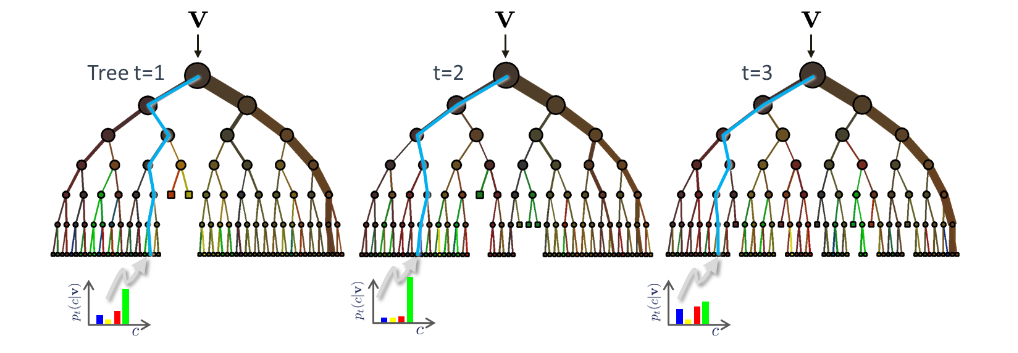
\includegraphics[width=0.9\linewidth]{images/forest}
\caption[Las decyzyjny.]{Schemat lasu decyzyjnego składającego się z trzech drzew \cite{criminisi2011decision}.}
\label{fig:forest}
\end{figure}
%TODO 2 też może rysunek

\item inne: np. SVM (ang. Support Vector Machine -- maszyna wektorów nośnych), AdaBoost itp.


\end{enumerate}

\section{Specyfikacja detekcji w podczerwieni}

Człowiek jest istotą żyjącą, co za tym idzie, wytwarza ciepło. Przeważnie ciało człowieka ma wyższą temperaturę niż otoczenie, co jest wyraźnie widoczne na obrazie termowizyjnym. Termowizja najlepiej sprawdza się w nocy, kiedy kontrast między człowiekiem a otoczeniem jest największy. Ta cecha powoduje, że podczerwień jest chętnie wykorzystywana do systemów wspomagania kierowcy, aby zwiększyć bezpieczeństwo poruszania się po drodze w nocy.  Sylwetka przechodnia może zostać w bardzo prosto wyodrębniona, wykonując prostą operację binaryzacji. Rysunek \ref{fig:binaryzacja} przedstawia przykładowy proces binaryzacji. Daje to możliwość zastosowania wielu algorytmów, które opierają się na kształcie obiektu (np. wzorzec probabilistyczny albo obliczenie proporcji wysokości do szerokości).

\begin{figure}[h]
	\centering
	\begin{subfigure}{0.47\textwidth}
		\centering
		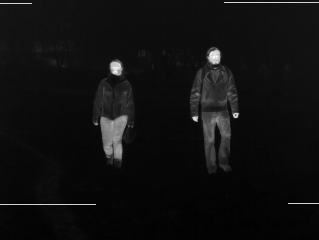
\includegraphics[width=0.9\linewidth]{images/Example_Oryginal}
		\subcaption{\label{fig:Example_Oryginal}}
	\end{subfigure}
	\begin{subfigure}{0.47\textwidth}
		\centering
		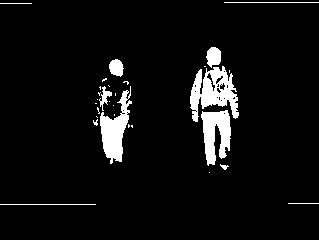
\includegraphics[width=0.9\linewidth]{images/Example_BW}
		\subcaption{\label{fig:Example_BW}}
	\end{subfigure}
	\caption[Przykład binaryzacji]{Binaryzacja: \protect\subref{fig:Example_Oryginal} Obraz zarejestrowany kamerą termowizyjną, \protect\subref{fig:Example_BW} Obraz po binaryzacji\cite{kankaing}.}
	\label{fig:binaryzacja}
\end{figure}

%TODO Nie omówił Pan specyfiki detekcji w podczerwieni.
%TODO 2 Czy specyfika detekcji w podczerwieni gdzies jest ?


\chapter{Wykorzystanie FPGA w analizie obrazu}
\label{cha:fpga}
Tradycyjne systemy wizyjne zwykle bazują na architekturze sekwencyjnej.
W tym rozwiązaniu obraz jest sukcesywnie poddawany kolejnym przekształceniom, a~wyniki pośrednie zapisywane są w pamięci operacyjnej. 
W aplikacji procesorowej operacje te są wykonywane przez układ arytmetyczno-logiczny. 
Kolejne kroki algorytmu są kompilowane w ciąg instrukcji dla procesora ,który oprócz operacji matematycznych dużą część pracy poświęca na pobieranie i dekodowanie rozkazów oraz na odczytywanie i zapisywanie danych do pamięci. 
By taka aplikacja mogła pracować w czasie rzeczywistym, cała procedura musi wykonać się szybciej niż przychodzące dane obrazu, co wymusza wysokie taktowanie procesora sięgające kilku GHz. To podejście jednak ma swoje ograniczenia. Wraz z wzrostem częstotliwości pracy procesora wzrasta jego moc a tym samym ilość ciepła które która musi zostać rozproszone. Najszybsze CPU są taktowane z częstotliwością zegara sięgającą nawet 4,4 GHz (choć przy zastosowaniu chłodzenia ciekłym azotem jest możliwe uzyskanie ponad 8 GHz). Wzrost szybkości obliczeń  uzyskuje się coraz częsciej poprzez zwiększanie ilości rdzen wi procesorze. %TODO dodać, że to i tak nie zawsze pomaga. Poza tym wypada jakoś skomentować fakt istnienie procesorów wielordzeniowych.

W przypadku podejścia równoległego, implementacja poszczególnych kroków algorytmu odbywa się w osobnych procesach. Jeżeli wykonywany algorytm jest głównie sekwencyjny tzn. kolejne kroki algorytmu wymagałyby danych otrzymanych z poprzednich, to zysk takiego zabiegu byłby równy zero. W celu uzyskania dobrej implementacji w układzie równoległym, istotne jest by znaczna cześć algorytmu mogła być wykonywana równolegle. 
%TODO OK to jest dość niejednoznaczne. Musi Pan to opatrzyć jakimś lepszym komentarzem/przykładem.
Maksymalne do uzyskania przyspieszenie jest określone przez prawo Amdahla: 
\begin{equation}
P_w =\frac{1}{ s + \frac{1-s}{n_w}}
\end{equation}
gdzie:
\begin{conditions}
P_{w} & przyspieszenie algorytmu w systemie wieloprocesorowym, \\
s & cześć algorytmu niepodlegająca zrównolegleniu (wartość od zera do jeden), \\
n_{w} & liczba elementów obliczeniowych.
\end{conditions}

Algorytmy przetwarzania obrazów są w dużej mierze równoległe, szczególnie te niskiego i średniego poziomu. W wielu przypadkach każdy piksel obrazu można obliczyć niezależnie, np. w wszelkich operacjach kontekstowych, przekształceniach przestrzeni barw, binaryzacji itp. Między innymi dlatego układy FPGA są chętnie stosowane w systemach wizyjnych. Teoretycznie jedynym ograniczaniem w możliwości zrównoleglenia obliczeń jest liczba dostępnych zasobów w układzie, jednak innym istotnym aspektem jest sposób dostarczania danych do modułów obliczeniowych. 
%TODO procesorów, czy modułów obliczeniowych no bo w sumie to musi się Pan ogólnie zdecydować, czy pisze to Pan ogólnie, czy z uwzględnieniem architektury.

Dostęp do pamięci często wymaga czasu a ilość danych przekazana podczas jednego transferu jest ograniczona. Stanowi to wąskie gardło w tego rodzaju rozwiązaniach.

% USUNIĘTE Czas i przepustowość jaka jest potrzebna do odczytania i zapisu obrazu po przetworzeniu pomiędzy pamięci jest najczęściej wąskim gardłem systemu wizyjnego. %TODO OK to z i do źle wygląda
Z tego powodu przetwarzanie obrazu bezpośrednio z sensora w czasie jego akwizycji jest chętnie wykorzystywane, gdyż zmniejsza to liczbę operacji odczytu i zapisu. \cite{garcia2014survey}

%TODO OK No i w ten sposób to Pan w rodziale o FPGA, ani razu nie użył słowa FPGA.
%TODO Druga sprawa to jest GPU - tez się tu powinno pojawić.


%TODO OK To trzeba wkomponować w rozdział o algorytmach. Ew. rozdział FPGA można dać przed algorytmy i wtedy omówić metody programowe oraz sprzętowe.

\section{Zynq-7000}

Rodzina układów Zynq-7000 bazuje na architekturze SoC (ang. \textit{System on Chip}). W pojedynczym układzie scalonym został zawarty kompletny system w skład którego wchodzą układy spełniające różne funkcje. Został on podzielony na dwie główne części: systemu procesorowy (PS ang. \textit{Porcessing System}) bazujący na procesorze ARM Cortex-A9 oraz logikę programowalną (PL ang. \textit{Programable Logic}) - FPGA. %TODO OK potworek styl. -> poprawić. + nazwy/słowa angielskie zawsze w kursywie
Na rysunku \ref{fig:zynq7000} przedstawiono schemat architektury układu. %TODO OK czego ?
Część procesorowa, oprócz samego ARM-a, posiada wbudowaną pamięć, kontroler pamięci zewnętrznej oraz szereg interfejsów dla układów peryferyjnych takich jak USB, GigEthernet, CAN, I2C, SPI. %TODO OK piwersza część do poprawy (styl.)
W części logiki programowalnej znajdują się bloki logiki konfigurowalnej (CLB ang. \textit{configurable logic block}), 36Kb bloki pamięci RAM, moduły DSP48, układ JTAG, układy zarządzania zegarami oraz dwa 12-bitowe przetworniki analogowo-cyfrowe.
%TODO 1. nie nazywałbym tego procesorem sygnałowym. 2. jednak bardziej obszerny opis obu komponentów (tak na 1/2 strony każdy)

Komunikacja między częścią procesorową, a logiką programowalną odbywa się za pośrednictwem interfejsu AXI (ang. \textit{Advanced Extensible Interface}) oraz bezpośrednio wykorzystując porty ogólnego przeznaczenia, przerwania i bezpośredni dostęp do pamięci (DMA ang. \textit{Direct Memory Access}).
%TODO 1. powt. oraz, 2 DMA, z tego co wiem, jest via AXI. Może chodziło Panu o ACP ?

\begin{figure}[h]
    \centering
    \includegraphics[width=1\textwidth]{images/Zynq-7000-Overview}
    \caption{Schemat ogólny architektury układu Zynq-7000.}
    \label{fig:zynq7000}
\end{figure}

\section{Interfejs AXI}
 AXI (ang. \textit{Advanced eXtensible Interface} --  zaawansowany rozszerzalny interfejs) jest częścią ARM AMBA (ang.\textit{ Advanced Microcontroller Bus Architecture}) -- otwartego standardu, będącego specyfikacją do zarządzania połączeniami między blokami funkcyjnymi w SoC. 
%TODO OK gdzie kończy się nawias ?
 Aktualnie jest stosowana AMBA 4.0 która wprowadziła drugą wersję AXI -- AXI4. 
 Występują trzy typy interfejsów dla AXI4:
\begin{itemize}
\item AXI4 -- stosowany w wysokowydajnych transferach w przestrzeni pamięci (ang. \textit{memory-mapped}),
\item AXI4-Lite -- stosowany dla prostszych operacji w przestrzeni pamięci (na przykład do komunikacji z rejestrami kontrolnymi i statusu),
\item AXI4-Stream --stosowany do transmisji strumieniowych (wysokiej prędkości). 
\end{itemize}
Specyfikacja interfejsu zakłada komunikację pomiędzy pojedynczym AXI \textit{master} i pojedynczym AXI \textit{slave}, która ma na celu wymianę informacji. 
Kilkanaście interfejsów AXI \textit{master} i \textit{slave} mogą zostać połączone między sobą za pomocą specjalnej struktury zwanej \textit{interconnect block} (blok międzypołączeniowy), w której odbywa się trasowanie połączeń do poszczególnych bloków. 

AXI4 i AXI4-Lite składają się z 5 różnych kanałów:
\begin{itemize}
\item Kanał adresu odczytu,
\item Kanał adresu zapisu,
\item Kanał danych odczytanych
\item Kanał danych do zapisania
\item Kanał potwierdzenia zapisu
\end{itemize}
Dane mogą płynąć w obie strony pomiędzy \textit{master} a \textit{slave} jednocześnie.
Ilość danych, które można przesłać w jednej transakcji w przypadku AXI4 wynosi 256 transferów, zaś AXI4-Lite pozwala na tylko 1 transmisję.

%TODO te słowa master i slave to kursywą.


AXI4-Stream nie posiada pola adresowego, a dane mogą być przesyłane nieprzerwanie. 
\chapter{Przegląd literatury}
\label{cha:przegLiter}

%TODO OK ponieważ te opisy są dość obszerne proszę jednak dać to w osobne podrozdziały subsub (czy jak to wyjdzie)

\section{Koledzy z Poznania}
W pracy \cite{kolzpoz} autorzy opracowali algorytm pozwalający na szybką i efektywną detekcję przechodniów w czasie rzeczywistym. 
Termowizja pozwala na uzyskanie dobrego kontrastu między poszukiwanym przechodniem a otoczeniem. 
Zaproponowany system jest dedykowany do pracy w nocy, kiedy kontrast między człowiekiem a otoczeniem pozwala na jednoznaczne ich rozróżnienie. %TODO OK między człowiekiem, a czym ?
Rozwiązanie bazuje na ulepszonym algorytmie progowania i segmentacji obrazu. 

Pierwszym etapem jest wyodrębnienie obszarów zainteresowań (ROI).
Pozwala to na znaczne ograniczenie obszaru analizowanych fragmentów obrazu. %TODO OK rozmiaru analizowanych fragmentów obrazu (czy jakoś tak)

Obraz w odcieniach szarości zostaję poddany binaryzacji z użyciem dwóch progów: mniejszym i większym. Pozwala to na detekcję przechodniów w różnych rejonach obrazu o różnym kontraście. 
Progi zmieniają się wraz z dynamiką obrazu wejściowego. 
W obrazie termicznym człowieka często w okolicy bioder znajduje się chłodniejszy obszar który jest poniżej progu binaryzacji co skutkuje przerwę między dwoma połówkami człowieka. Aby połączyć je w jedną całość dodatkowo dla każdego obszaru wyłonionego podczas binaryzacji zostają wytypowane dodatkowe ROI, które obejmuje ten obszar wraz z innymi znajdującymi się nad lub pod. 
%TODO OK OK1. powt. dod, 2. niejasen
%TODO OK Proszę to kwestię dwóch progów lepiej opisać. Bo nie wiadomo jak co i po co jest robione.
%TODO OK to "tworząc" coś nie pasuje
%TODO OK to też jest niejasne. 
%TT przepisałem ten akapit

Następnym krokiem jest filtracja wyników. 
Ma ona na celu zredukowanie liczby obszarów przed końcową analizą. 
Autorzy zastosowali filtrację opierającą się na proporcji obszaru zainteresowań. 
Pozytywnie zakwalifikowane zostały tylko obszary o odpowiednich proporcja wysokości do szerokości (1:1.3 do 1:4). 
Z racji, że badany obraz pochodzi z kamery zamontowanej na stałe na samochodzie, autorzy wykorzystali filtrację perspektywiczną która uwzględnia możliwą wysokość ROI w różnych fragmentach obrazu. %TODO OK tu jest coś nie tak...
Filtracja jednorodnych regionów pozwoliła na odrzucenie kandydatów będących częścią szerszych obiektów nie mających nic wspólnego z przechodnimi. Obraz człowieka cechuje się dużą rozpiętością wartości temperatur. Obliczając odchylenie standardowe ROI w odcieniach szarości można wyeliminować obszary które są poniżej progu określonego przez autorów.  %TODO OK To jest niejasne...

Ostatnim krokiem algorytmu jest klasyfikacja wytypowanych kandydatów. 
Autorzy wykorzystują histogram zorientowanych gradientów jako deskryptor tworząc wektor 3780 cech, które są następnie klasyfikowane przez SVM.

W celu zbadania dokładności algorytmu został przeprowadzony test na zbiorze CVC-14, który zawiera obrazy nagrane kamerą FIR podczas nocnego przejazdu samochodem. 
Testy wykazały, że metoda podwójnego progowania daje trzy razy lepsze rezultaty, niż przy wykorzystaniu pojedynczego progu.  Wraz z zaproponowanymi technikami filtracji zaowocowało to bardzo efektywnym mechanizmem segmentacji. Ponad 95\% występujących przechodniów zostało poprawnie wytypowanych jako kandydaci do klasyfikacji. 
%TODO ok no właśnie segmentacji czy klasyfikacji
Cała procedura detekcji przechodniów osiągnęła wysoki poziom wydajności na poziomie 33 klatek (o wymiarach 640x471 px) na sekundę przy wykorzystaniu pojedynczego rdzenia CPU. Dokładność detekcji wyniosła 37,3\% AMR
(ang. \textit{ average miss rate }), co jest porównywalna do innych metod opartych o HOG+SVM.
%TODO A dla jakich parametrów strumienia wizyjnego. 
%TT nie jest napisane wprost w artykule ale mam tą samą bazę i tam są 640 x 471.

\section{Stereotermowizja}
W pracy \cite{suard2006pedestrian} autorzy zaproponowali wykorzystanie dwóch kamer termowizyjnych tworząc system stereowizyjny. W obrazie termowizyjnym człowieka najcieplejszym obszarem jest zazwyczaj głowa. By wyodrębnić obszary zainteresowania, w~których potencjalnie znajdują się przechodnie, zgrupowano piksele o wartościach powyżej kilku różnych progów. Każdy z tych obszarów zostaje następnie uznany za głowę i stanowi górną część okna detekcyjnego. Wielkość okna jest estymowana na podstawie odległości źródła ciepła od kamer.. Odległość jest ustalana na podstawie mapy dysparycji (ang. \textit{disparity map}). Do obliczani dysparycji okna, porównywana różnica między oryginalnym oknem a oknem przesuwnym w drugim obrazie. Dysparycja jest uzyskiwana gdy ta różnica jest minimalna. Na koniec każde okno zostaje przeskalowane do wielkości 128x64 i poddane klasyfikacji . %TODO OK znowu za mało szczegółów...
%TODO OK to raczej, z tego że ZWYKLE głowa (stricte twarz) ew. dłonie sa odsłoniete, wynika, że są widoczne jako najcieplejsze... bo tak ogólnie to chyba temperatura jest względnie równomiarna.

W tej pracy autorzy skupili się na optymalnym doborze parametrów deskryptora HOG. 
Zestaw zawierał 4400 obrazów: 2200 próbek z pieszymi oraz 2200 bez pieszych. 
Został wykorzystany następujący zestaw parametrów HOG:
\begin{table}[!h]
\centering 
\begin{threeparttable}
\caption{Parametry HoG.}
\label{tab:parametryhog}
\begin{tabularx}{1\textwidth}{|l|X|X|}


\hline Parametr & Zestaw do testów & Najlepszy wynik \\ 
\hline Rozmiar komórki & 4x4, 8x8, 16x16 & 8x8 \\ 
\hline Rozmiar bloku & 1x1, 2x2, 4x4 & 2x2 \\ 
\hline Nakładanie się komórek między blokami & 1,2 & 1 \\ 
\hline Schemat normalizacji bloków & brak, L1, L2 & L2 \\ 
\hline Liczba przedziałów histogramu & 4, 8, 16 & 8 \\ 
\hline Rodzaj histogramu & ważony, nie ważony & ważony \\ 
\hline 


\end{tabularx} 
\end{threeparttable}
\end{table} 

%TODO Wnioskuję, że to liniowy SVM był - proszę to jawnie napisać.
Autorzy przeprowadzili po 10 procedur uczenia klasyfikatora dla każdej kombinacji wykorzystując różne kombinacje danych do nauki i testów. W tabeli \ref{tab:parametryhog} zaprezentowane są wyniki badań.

Badanie parametrów dla klasyfikacji SVM wykazało, że im większy zestaw uczący tym lepszą można uzyskać skuteczność detekcji. 




%TODO Opis tego trzeciego algorytmu jest to poprawki !!! %TT jest zbędny więc usunięty
% \section{Do wywalenia}
% Autorzy pracy \cite{nanda_2002} przedstawili metodę opartą o wzorzec probabilistyczny i klasyfikator Bayesa. 
% Obraz wejściowy zostaje zbinaryzowany z zadanym progiem. 
% Próg ten nie jest stały i zależy od wielu czynników. 
% %TODO a można konkretniej ? Np., że zostało to omóione poniżej
% Autorzy bazując na danych uczących stanowiących 1000 prostokątnych okien o rozmiarze 48x128 pikseli zawierających przechodnia średnią oraz odchylenie standardowe wartości dla pikseli należących do obrazu przechodnia \( \mu_1 \sigma_1 \) bądź tła \( \mu_2 \sigma_2 \) a następnie obliczyli próg binaryzacji za pomocą równia \eqref{eq:treshold_nanda}. %TODO OK odwołania do równiań poprzez eqref. , te symbole jakoś w tekście nie są w nawiasie
% %TODO To zadnie to jest jakiś "potworek" proszę poprawić.
% 
% \begin{equation} \label{eq:treshold_nanda}
% threshold = \frac{\sigma_1 \sigma_2}{ \sigma_1 + \sigma_2} \ln\left ( \frac{\sigma_1}{\sigma_2} \right ) + \frac{\sigma_1\mu_1 + \sigma_2\mu_1}{\sigma_1+\sigma_2}\end{equation}
% 
% Aby uzyskać wzorzec prawdopodobieństwa, zbiór testowy został zbinaryzowany z uprzednio wyliczonym progiem. 
% Następnie zostało obliczone prawdopodobieństwo przynależności piksela do przechodnia we wzorcu. %TODO To jest ciut niejasne.
% Mając już wzorzec, został obliczony combinedpropability ze wzoru \eqref{eq:combo_nanda} dla 1000 okien zawierających i nie zawierających człowieka oraz wyciągnięta średnia i odchylenie standardowe dla nich. 
% 
% %TODO To com.... to trzeba na coś zamienić !!!
% 
% Dało to podstawę do obliczenia progu dla wartości combinedpropability z wzoru \eqref{eq:treshold_nanda}. 
% %TODO to jest jakieś niejasne.
% 
% \begin{equation} \label{eq:combo_nanda} combinedprobability(i,j)=\sum_{x=1}^{48}\sum_{y=1}^{128}(th(x,y)*p(x,y)+(1-th(x,y))*(1-p(x,y)))\end{equation}
% \noindent
% gdzie \(th(x,y)\) to okno wokół piksela \((i,j)\), a \(p(x,y)\) to wzorzec prawdopodobieństwa wystąpienia pieszego.
% 
% Badana klatka obrazu jest badana poprzez okno przesuwne tworząc mapę prawdopodobieństwa. %TODO badana klatka jest badana ? 
% Wartości które przekroczą próg wskazują, że w danym oknie znajduje się człowiek. 
% 
% %TODO ale jakie wartości ? 
% Autorzy zbadali algorytm na 6 sekwencjach filmowych i uzyskali wynik między 75\%-90\% wykrycia przy jednym fałszywym wykryciu na ramkę. %TODO chyba średnio jednym...

%TODO Tutaj omówienie tych algorytmów z Poznania

\section{Podejście sprzętowo-programowe. Stereowizja dla robotów }

W pracy \cite{honegger2014real} autorzy wykorzystali układ FPGA oraz CPU małej mocy do skonstruowania systemu wizyjnego dla robotów. 
System analizował obraz stereoskopowy z dwóch kamer wizyjnych tworząc mapę głębi. 
\begin{figure}[h]
    \centering
    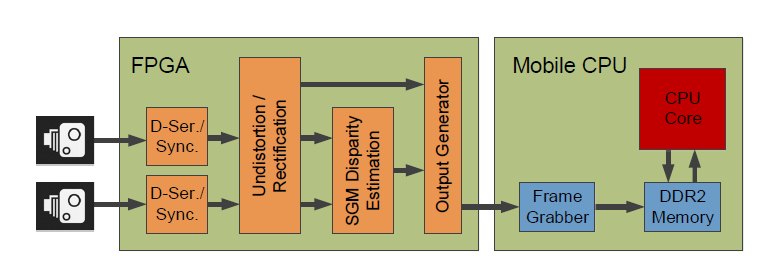
\includegraphics[width=1\textwidth]{images/honegger2014real_Fig1}
    \caption{Schemat systemu wizyjnego zaproponowanego w pracy\cite{honegger2014real}.}
    \label{fig:honegger2014real_Fig1}
\end{figure}
%TODO OK wizyjnych, czy termo
Obie kamery zostały bezpośrednio podpięte do układu FPGA za pomocą interfejsu LVDS (ang. \textit{low-voltage differental signal} – niskonapięciowy sygnał różnicowy), w którym obrazy były następnie przetwarzane. 

%TODO OK proszę zwrócić uwagę na czas -> były (bo wcześniej wykorzystali) ogólnie takie badania opisuje się w czasie przeszłym.

Schemat systemu jest przedstawiony na rysunku \ref{fig:honegger2014real_Fig1}. W pierwszej kolejności obrazy z kamer są synchronizowane z wykorzystaniem bufora opóźniającego jedną linie danych. 
Korekcja zniekształceń soczewkowych oraz rektyfikacja zostały połączone w jedną operację. Przychodzące zsynchronizowane piksel są zapisywane do bufora. Po obliczaniu współrzędnych piksela, uwzględniającym korektę, jego wartość jest pobrana z właściwej lokalizacji w buforze wejściowym. Kolejnym krokiem było obliczanie dysparycji. W tym celu kontekst piksela z lewego obrazu jest porównywany z okolicznymi kontekstami pikseli w prawym obrazie. Kandydat jest wyłaniany na podstawie lokalnej funkcji kosztu i stałych globalnych bazujących na algorytmie SGM (ang. \textit{Semi-Global Matching}). 

Następnie dwa oryginalne obrazy oraz mapa głębi są przesyłane do CPU za pomocą specjalnej magistrali.
%TODO OK może magistrali
Moduł \textit{frame grabbera} przechwytywał ten obraz i wykorzystując DMA (ang. \textit{Direct Memeory Acces}) zapisywał do pamięci systemu.
%TODO OKno to jest niejasne... tzn. ta pierwsza część zdania.
System pracował w rozdzielczości 752x480 pikseli i 60 klatkach na sekundę. 
Całość, włącznie z kamerami, układem FPGA, CPU oraz konwerterami napięcia pobierał mniej niż 5W mocy. 
Całkowita latencja podana przez autorów rozwiązania wynosi około 2ms.

%TODO ale to coś jeszcze robiło ? Bo rozumiem, że FPGA liczyło stereo (pytanie jak) i do CPU trafiały te obrazy. Ale coś więcej się działo ? 
%TT niestety nie, po prostu szybko liczyło obraz stereo z wykorzystaniem fpga

\section{Podejście sprzętowo-programowe. System wspomagania kierowcy}
W pracy \cite{piao2016real} autorzy wykorzystali układ SoC (ang. System on Chip) do detekcji pieszych dla zaawansowanego systemu wspomagania kierowcy (ADAS ang. \textit{advanced driver assistance system}). 
Głównym wyzwaniem było opracowanie systemu, która działa w czasie rzeczywistym, ma mały pobór mocy oraz niski koszt wykonania. 
%TODO OK raczej systemu/rozwiązania (szczególnie koszt wykonania dla algorytmu jest dyskusyjny)
Najbardziej skuteczne algorytmy wymagają znacznych zasobów obliczeniowych. %TODO topowych -> słowo potoczne i do zmiany
Autorzy dokonali zatem relaksacji problemu poprzez zastosowanie prostszego deskryptora jakim jest LBP oraz klasyfikatora SVM. 
Po każdej stronie pojazdu została zamontowana inteligentną kamerę o szerokim, 180$^\circ$ horyzontalnym kącie widzenia by jak najlepiej monitorować przestrzeń wokół niego. 
%TODO wyeliminiować powt. autorzy
W kamerach została przeprowadzona wstępna obróbka obrazu (rektyfikacja i skalowanie). 
%TODO rektyfikacja ? czyli to był system stetero ?
%Nie był to system stereo ale w artykule wyraźnie piszą o rektyfikacji, choć podejrzewam że chodziło im o korekcje soczewkową 
Przetworzony obraz z kamer był transmitowany do \textit{,,Fusion-Box''}, gdzie odbywała się generacja kandydatów, klasyfikacja, weryfikacja oraz śledzenie. 
Wyniki były przesyłane do wbudowanego komputera PC. 
Rozwiązanie nie zostało jeszcze w pełni zaimplementowane, ale pierwsze testy dawały obiecujące rezultaty.

\section{Wzorzec probabilistyczny}
\label{sec:xiao_2015}
W pracy \cite{xiao_2015} autorzy wykorzystali układ FPGA i naiwny klasyfikator Bayesa do detekcji przechodniów w obrazie termowizyjnym. Klasyfikator zakłada, że wszystkie predykatory są niezależne od siebie co znacznie upraszcza obliczenia. Za pomocą tego klasyfikatora można określić przynależność obrazu w badanym oknie do jednej z dwóch klas: zawierającego przechodnia albo nie zawiera (czyli tła). W tym przypadku predykatorami są poszczególne piksele. Dla każdego piksela w oknie określa się prawdopodobieństwo jego przynależności do danej klasy. Klasyfikacja sprowadza się do zależności \eqref{eq:bayes_china}.
%TODO OK do za ??? poza tym to jest coś niejasne}
%TT opis poprawiony

\begin{equation} \label{eq:bayes_china}
\sum_{x,y} \ln p(w_{x,y}|P) > \sum_{x,y} \ln p(w_{x,y}|\bar{P})
\end{equation}

\noindent gdzie \( p(w_{x,y}|P) \) to prawdopodobieństwo że piksel $w_{x,y}$ przynależy do obrazu człowieka
\( p(w_i|\bar{P}) \) przynależy do tła.
%TODO no ale co to jest i, bo czegoś tu nie rozumiem....
Jeżeli nierówność jest prawdziwa wtedy okno zostaje sklasyfikowane jako zawierające przechodnia.
Obrazy wykorzystane w systemie są binarne, co oznacza że \( p(w_{x,y}|P) \) przyjmuje dwie wartości, w zależności czy jest to piksel czarny czy biały. Można w ten sposób stworzyć macierz rozkładu prawdopodobieństwa (PDM ang. \textit{probability distribution matrix})która określa prawdopodobieństwo wystąpienia białego piksela w oknie (prawdopodobieństwo wystąpienia czarnego jest \(1-  p(w_{x,y}|P) \)). Inną nazwą tej macierzy jest wzorzec probabilistyczny.
Autorzy utworzyli PDM na podstawie 60 pozytywnych próbek. 

W celu usprawnienia obliczeń w układzie FPGA macierz została przeskalowana na wartości całkowitoliczbowe w zakresie od 1 do 127. 
Następnie obliczono logarytm o podstawie dwa z uzyskanego wzorca i jej odwrotności (poprzez odjęcie od 128 wartości macierzy pozytywnej) i pomnożono przez 32. %TODO OK powt. następne
Utworzono tak dwie macierze: LPDW i LPDB dla białych i czarnych pikseli. (ang. \textit{logarithmic probability matrix} – logarytmiczna macierz prawdopodobieństwa). 
Przyjęto, że prawdopodobieństwo przynależności piksela do tła jest stałe i wynosi 50\%, co daje wartość 192 po uprzednich przekształceniach. 
Ostatecznie klasyfikacji dokonuje się z wzoru: 
%TODO OK raczej klasyfikacji dokonuje się...

\begin{equation}\label{equ:Lp}
L_{p} = \sum_{x=1}^{j}\sum_{y=1}^{k}(th(x,y)*LPMW(x,y)+(1-th(x,y))*LPMB(x,y))
\end{equation}
\begin{equation}\label{equ:Lb}
L_{b} = j*k*192
\end{equation}
\begin{equation} \label{equ:ispedistant}
IsPedestrian = \left\{ \begin{array}{ll}
1 & \textrm{gdy $L_{p} \geq L_{b} + K$}\\
0 & \textrm{gdy $L_{p}<L_{b} + K$}
\end{array} \right.
\end{equation}

\noindent gdzie $j$ i $k$ stanowią wysokość i szerokość okna przesuwnego. Wartości $L_p$ i $L_b$ odnoszą się do sum prawdopodobieństw przynależności białego/czarnego piksela do obrazu człowieka. $K$ jest parametrem którym określono minimalną wartość dla której klasyfikator daje poprawne pozytywne wyniki.

W omawianej pracy autorzy opracowali wzorce dla 3 różnych wielkości okna: 10x15, 8x12 i 6x9 pikseli. Do stworzenia wykorzystali jedynie górne połówki obrazu termicznego ludzkiej sylwetki, co miało na celu bardziej niezawodnego wzorca wobec różnych postur przechodniów. 
\section{Poprzednie prace}
Praca inżynierska \cite{kankaing}, oraz artykuł na jej podstawie\cite{kanka2016fpga}, której kontynuacją jest mniejsza praca, rozwinęła koncepcję zaproponowaną w sekcji \ref{sec:xiao_2015}. Zastosowano 4 wzorce o wymiarach 48x120, 32x80, 24x60,19x48. Wzorzec został podzielony na 4 części: górną, dolną , prawą lewą. Następnie, podobnie jak w DPM, układ tych 4 części decydował o jego klasyfikacji. Każda część tworzyła maskę wielkości całego okna. Jeżeli co najmniej 3 takie maski pokrywały się obszar ten był klasyfikowany pozytywnie. Pozwoliło to na znaczną poprawę działania algorytmu, co pokazuje wykres ROC przedstawiony na rysunku \ref{fig:analiza_wykres}. 

	\begin{figure}
	\centering
	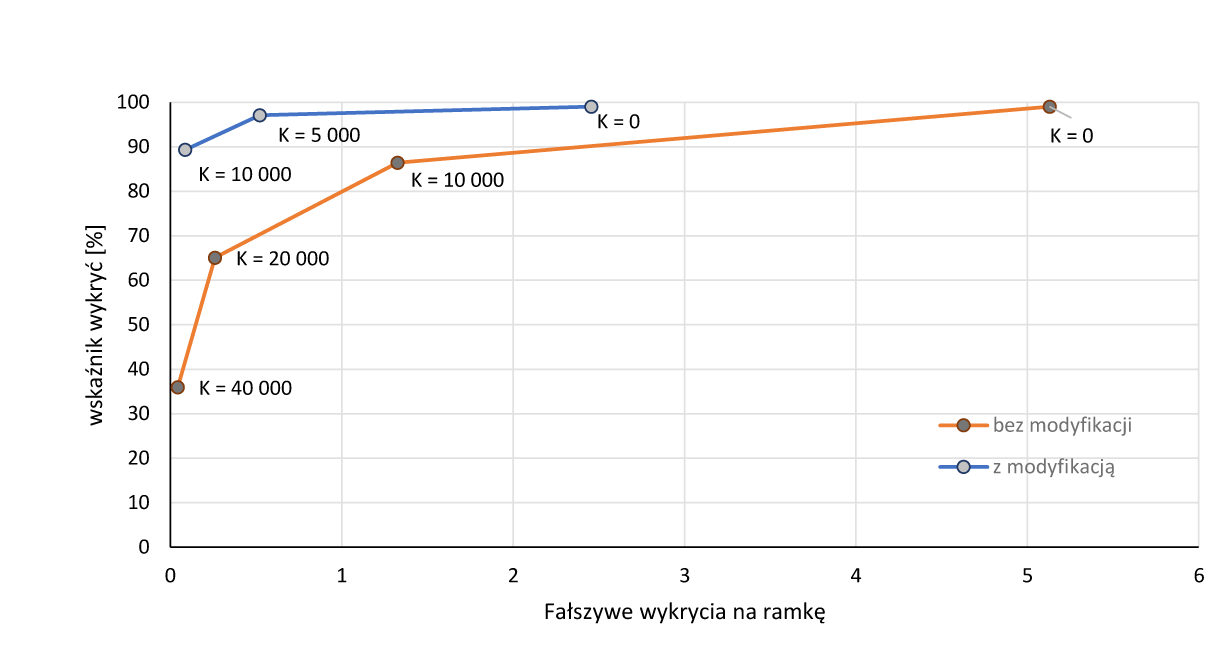
\includegraphics[width=0.8\linewidth]{images/Analiza_wykres}
	\caption[Wykres REC]{Wyniki symulacji przy różnych wartościach parametru K.}
	\label{fig:analiza_wykres}
	\end{figure}

Poprawiło to również detekcję w różnych skalach. Poprzednio \textit{muliscale} osiągnięto dzięki zastosowaniu kilku wzorców. Pojedyńczy wzorzec zapewniał detekcję w pewnym zakresie wysokoci przechodniów. Im dalej odniegiał od swojej nominalnej wysokoci tym bardziej należało zmniejszyć parametr $K$ by w pojedynczym oknie było możliwe wykrycie mniejszych i większych sylwetek. Powodowało to również zwiększenie ilości fałszywych detekcji. Po wprowadzeniu modyfikacja każda część ma możliwość deformacji co w dynamiczny sposób pozwala na zmianę wysokości wzorca.

%TODO OK ogólnie ta metoda (z p. inż. też jest jakoś nie do końca fajnie opisana) - proszę to dopracować.
%TODO OK dalej - proszę "pochwalić" się artykułem na ten temat - przecież powstał





\chapter{Zrealizowany system wizyjny} %TODO 2 napisać do czego...
\label{cha:propSysWiz}

\begin{figure}
\centering
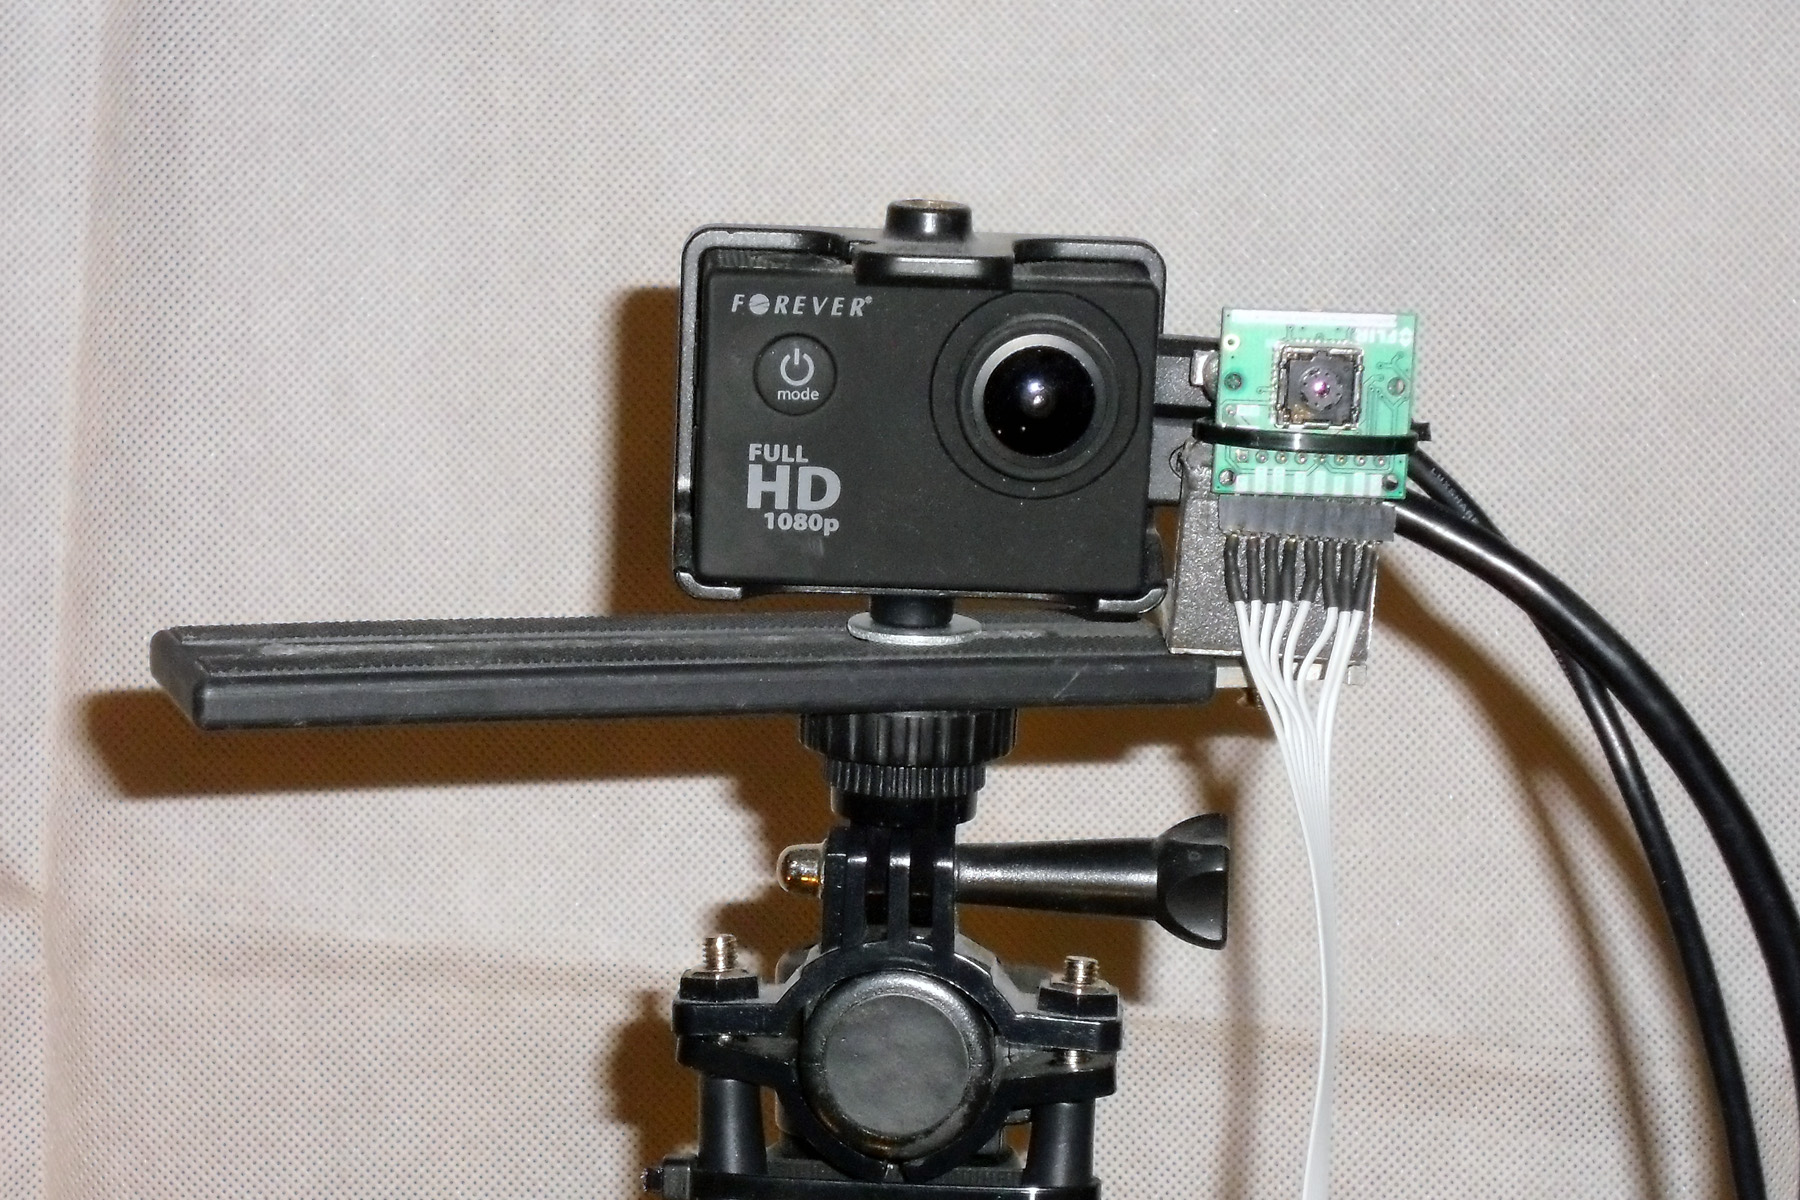
\includegraphics[width=0.65\linewidth]{images/kameraRGBIR.jpg}
\caption[Wykorzystany system kamer.]{Wykorzystany system kamer. Po lewej stronie znajduje się kamera wizyjna, po prawej termowizyjna Lepton.}
\label{fig:kameraRGBIR}
\end{figure}

\begin{figure}
\centering
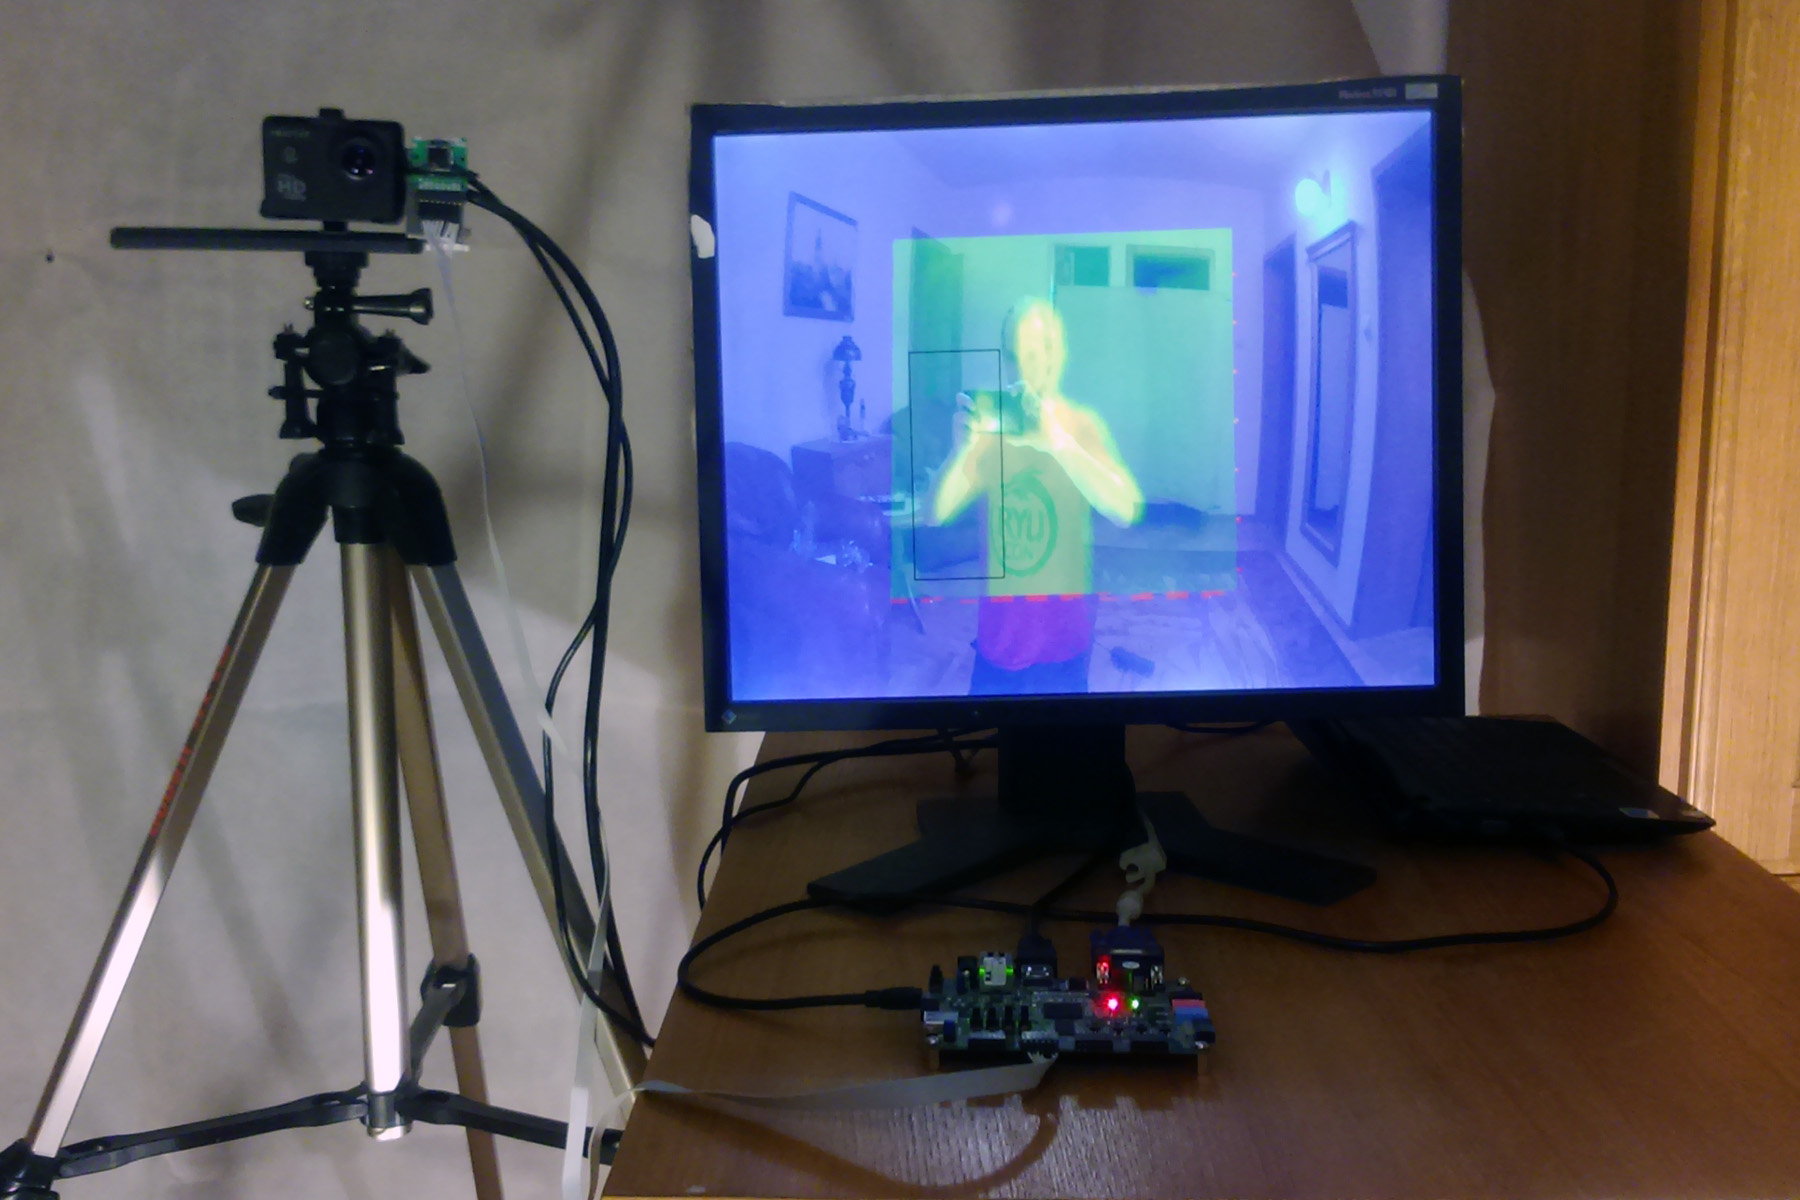
\includegraphics[width=0.65\linewidth]{images/systemOverview.jpg}
\caption[Widok na kompletny system.]{Widok na kompletny system do detekcji obiektów w przestrzeni multispektralnej. Obraz jest rejestrowany przez zespół kamer znajdujący się na statywie. Kamery są połączone do płytki deweloperskiej Zybo. Wynik jest prezentowany na monitorze.}
\label{fig:systemOverview}
\end{figure}

\section{Koncepcja systemu}

Zadaniem systemu jest detekcja osób na obrazie multispektralnym. 
Do uzyskania obrazu multispektralnego została wykorzystana kamera wizyjna, dająca obraz o~rozdzielczości 640x480 pikseli i~50 klatek na sekundę oraz termowizyjna: Lepton -- 80x60 pikseli i~9 klatek na sekundę. 
Obraz z~kamery termowizyjnej (IR) jest dopasowywany do wizyjnego (RGB) za pomocą projekcji perspektywicznej. 
Wynikiem ich połączenia jest obraz multispektralny (RGBIR). 
Wybór ROI odbywa się tylko z wykorzystaniem obrazu termowizyjnego. 
W~tym celu został wykorzystany moduł PDM (ang. \textit{Probability Density Matrix}) zaczerpnięty z pracy inżynierskiej autora \cite{kankaing}.
Tworzy on listę kandydatów, z której jest wybierany najbardziej prawdopodobny wynik. 
Następnie z ROI o wymiarach 80x192 piksele wyodrębniane są deskryptory HOG oraz przeprowadzana jest klasyfikacja z wykorzystaniem SVM. 
Wynik detekcji jest prezentowany na ekranie, poprzez obramowanie sylwetki przechodnia.
Do realizacji tego systemu została wykorzystana płytka deweloperska ZYBO firmy Digilent. 
Bazuje ona na omówionym wcześniej w~rozdziale \ref{cha:fpga} układzie Zynq-7000. 
Jest to układ heterogeniczny, co daje możliwość realizacji poszczególnych elementów systemu wizyjnego w~logice programowalnej (PL) lub systemie procesorowym (PS)
Zaproponowano następujący podział zadań:

Logika programowalna:
\begin{itemize}
\item Akwizycja obrazu poprzez HDMI (RGB) i VoSPI (IR),
\item Transformata projekcyjna i interpolacja obrazu IR,
\item Nałożenie i synchronizacja obrazu IR do obrazu RGB,
\item Prezentacja wyników,
\item Detekcja kandydatów za pomocą wzorca probabilistycznego.
\end{itemize}
System procesorowy:
\begin{itemize}
\item konfiguracja parametrów systemu wizyjnego w~logice programowalnej poprzez interfejs AXI4-Lite,
\item Klasyfikacja obszarów wytypowanych przez wzorzec probabilistyczny (HOG+SVM),
\item Generowanie wyników.
\end{itemize}
\begin{figure}[h]
\centering
\includegraphics[width=1\textwidth]{images/system}
\caption{Schemat blokowy systemu detekcji.}
\label{fig:systemwizyjny}
\end{figure}

Na rysunku \ref{fig:systemwizyjny} został przestawiony ogólny schemat rozwiązania.

\section{Model programowy}

W~celu sprawdzenia koncepcji systemu została wykonana jego implementacja w~pakiecie Matlab. 
Do testów został wykorzystany zestaw filmów pochodzący z~pracy \cite{bilodeau2014thermal}. 
Przestawia on pomieszczenie, po którym porusza się od 1~do 5~aktorów. 
Obraz został nagrany dwoma kamerami: termowizyjną FLIR Thermovision A40M oraz wizyjną Sony XCD-710CR. 
Rozdzielczość obu klipów wynosi 480x360 piksele. 
W~pierwszym etapie obraz z~kamery termowizyjnej został pomniejszony do rozmiarów 80x60 piksele. 
Następnie, za pomocą wzorca probabilistycznego o~wymiarze 30x12 piksele została obliczona mapa rozkładu LP na obrazie jak na rysunku \ref{fig:sampleLP}. %TODO 2 co to jest LP ? 
Maksima lokalne występujące w tym rozkładzie stanową środki ROI do dalszej analizy (rysunek \ref{fig:sampleTemplateDetection}).
\begin{figure}[h]
\centering
\begin{subfigure}{0.32\textwidth}
\centering
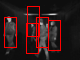
\includegraphics[width=0.9\linewidth]{images/sampleTemplateDetection}
\subcaption{\label{fig:sampleTemplateDetection}}
\end{subfigure}
\begin{subfigure}{0.32\textwidth}
\centering
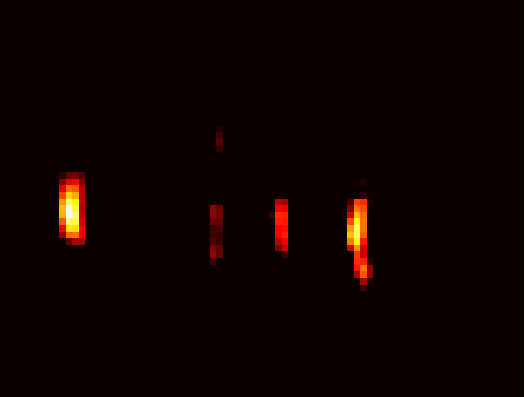
\includegraphics[width=0.9\linewidth]{images/sampleLP}
\subcaption{\label{fig:sampleLP}}
\end{subfigure}

\caption[Poszukiwanie kandydatów za pomocą wzorca probabilistycznego.]{Poszukiwanie kandydatów za pomocą wzorca probabilistycznego. \protect\subref{fig:sampleTemplateDetection} wytypowani kandydaci \protect\subref{fig:sampleLP} mapa LP.}
\end{figure}

Obraz termowizyjny został dopasowany do obrazu wizyjnego, tworząc obraz multispektralny. 
Punkty kalibracyjne zostały wyznaczone na podstawie elementów sylwetek (stopy, dłonie i głowa) od aktorów których wysokość na obrazie wynosiła około 180 pikseli. 
Zmniejsza to do minimum dysparycję dla obiektów poszukiwanych wzorcem o~wysokości 30 pikseli. %TODO 2 dla mnie to zdanie jest niejasne
Następnie punkty znalezione podczas badania wzorcem probabilistycznym zostały przeniesione na obraz multispektralny z~wykorzystaniem parametrów transformacji uzyskanej podczas kalibracji. 
Wokół tych punktów zostały wyznaczone ROI o~wymiarach 80x192 pikseli.
%TODO 2 a można zdanie więcej jak dokładnie... 
Dalej został obliczony wektor cech HOG w każdym z okien, które następnie zostały poddane klasyfikacji za pomocą liniowego SVM.
\begin{figure}[h]
\centering
\begin{subfigure}{0.32\textwidth}
\centering
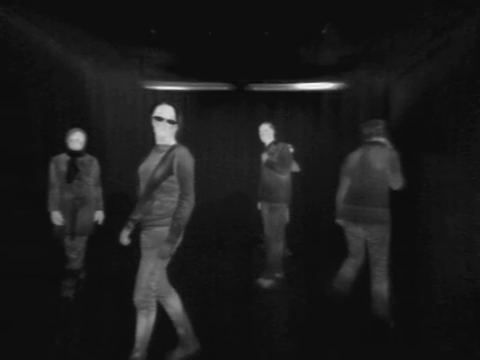
\includegraphics[width=0.9\linewidth]{images/sampleIR}
\subcaption{\label{fig:sampleIR}}
\end{subfigure}
\begin{subfigure}{0.32\textwidth}
\centering
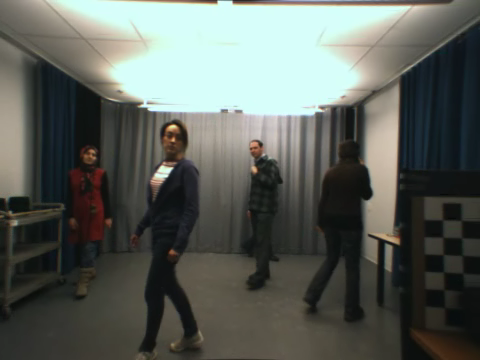
\includegraphics[width=0.9\linewidth]{images/sampleRGB}
\subcaption{\label{fig:sampleRGB}}
\end{subfigure}
\begin{subfigure}{0.32\textwidth}
\centering
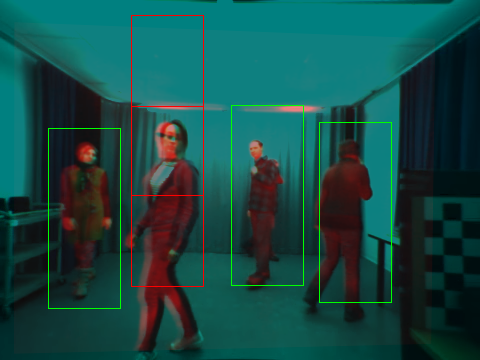
\includegraphics[width=0.9\linewidth]{images/sampleHOGSVM}
\subcaption{\label{fig:sampleHOGSVM}}
\end{subfigure}

\caption[Detekcja]{\protect\subref{fig:sampleIR} Obraz z kamery termowizyjnej, \protect\subref{fig:sampleRGB} obraz z kamery wizyjnej, \protect\subref{fig:sampleHOGSVM} połączone obrazy z zaznaczonymi wynikami detekcji. Zielona ramka oznacza pozytywny wynik klasyfikacji HOG SVM, czerwona -- negatywnie sklasyfikowani kandydaci.}
\end{figure}

Do nauczenia SVM zostały wykorzystane 141 ROI wytypowanych przez wzorzec probabilistyczny. 
Każdemu ROI została przypisana klasa: 1 -- jeżeli zawiera obraz człowieka o~wysokości 160+/-20 px , 0 -- jeżeli jest to element tła bądź część człowieka (np. sama głowa, nogi).

Na 141 próbek 78 stanowiły próbki pozytywne a~62 negatywne. 
SVM sklasyfikował poprawnie pozytywnie 88,9\% próbek zaś poprawnie negatywnie 88,5\%.

%TODO 2 w sumie mało próbek, ale .... trudno

\section{Wykorzystanie AXI-Stream do transmisji sygnału wideo.}

W odróżnieniu od standardowego sposobu przetwarzania strumieniowego wideo, w~AXI4-Stream przesyłane są jedynie aktywne piksele.
Linie synchronizacji poziomej i~pionowej są odrzucane albo przekierowywane do specjalnego bloku, w~którym są mierzone parametry wchodzącego strumienia wizyjnego (liczba pikseli w~linii, liczba aktywnych linii, czas wygaszania itd.).
W~celu wyświetlenia obrazu wykorzystuje się ten sam blok, który ma możliwość generacji nowych sygnałów synchronizacji (ich odtworzenia).

Do transmisji wykorzystane jest 6 sygnałów: dane i~pięć kontrolno-sterujących. 
W~nawiasach są podane linie, które wykorzystuje dany sygnał w~interfejsie AXI4-Stream.
\begin{itemize}
\item \textit{Video Data} (\textit{tdata})-- linia danych o szerokości jednego (albo dwóch) pikseli. Szerokość tej linii powinna być wielokrotnością liczby osiem (16, 24, 48 itd.)
\item \textit{Valid}(\textit{tvalid}) -- linia określająca czy dane piksela są poprawne,
\item \textit{Ready} (\textit{tready})-- linia kontrolna informująca urządzenie master, że \textit{slave} jest gotowy do transmisji danych, 
\item \textit{Start Of Frame} (\textit{tuser}) -- linia sygnalizacyjna pierwszego piksela nowej ramki,
\item \textit{End Of Line} (\textit{tlast})-- linia sygnalizacyjna ostatniego piksela w~linii. 
\end{itemize}

Aby mógł wystąpić poprawny transfer danych linie \textit{Valid} i~\textit{Ready} muszą być w stanie wysokim podczas rosnącego zbocza zegara.
Przykładowe nawiązanie transmisji przedstawia rysunek \ref{fig:handshake}.

\begin{figure}[h]
\centering
\includegraphics[width=1\textwidth]{images/axi-stream_hendshake}
\caption{Przykład rozpoczęcia transmisji Ready/Valid.}
\label{fig:handshake}
\end{figure}


\section{AXI VDMA}
Wiele aplikacji wizyjnych wymaga przechowania całej ramki obrazu w~celu jej dalszej obróbki np. podczas skalowania, przycinania bądź dopasowania liczby klatek na sekundę.
Część programowalna układu Zynq zazwyczaj nie posiada wystarczającej liczby wewnętrznych zasobów pamięciowych do przechowania pełnej klatki obrazu.
Aby stworzyć taki bufor jedną z~możliwości jest wykorzystanie mechanizmu bezpośredniego dostępu do pamięci, który pozwala na przesłanie i~wczytanie danych z logiki programowalnej do pamięci RAM bez konieczności angażowania procesora.
Należy w~tym miejscu zaznaczyć, że dla rozważanej platformy Zybo zewnętrzna pamięć RAM DDR podłączona jest do kontrolera w~systemie procesorowym.

Dostęp ten realizuje się poprzez IP-Core AXI VDMA.
Zapewnia on przejście między interfejsem AXI4-Stream, a~AXI4 Memory Map w~obu kierunkach.
Przed rozpoczęciem przesyłania IP-Core jest konfigurowany poprzez interfejs AXI4-Lite.
Konfiguracja zawiera adres w pamięci RAM do którego ma być zapisana bądź wczytana ramka obrazu.
Po wgraniu do pamięci ramki kontroler może wywołać przerwanie dla systemu procesorowego.

\section{Opis modułów zaimplementowanych w~logice programowalnej}

\subsection{Kontroler kamery IR}
Kamera Lepton przesyła obraz za pomocą interfejsu VoSPI (ang. \textit{Video over Serial Peripheral Interface}). 
W~zastosowanym rozwiązaniu jest on urządzeniem typu \textit{slave}, zaś układ Zynq jest \textit{masterem}. 
Są wykorzystywane 3 z~4 linii typowego kanału SPI: SCK (ang. \textit{Serial Cloack} -- zegar), /CS (ang. \textit{Chip Select} -- wybór układu)(aktywny stanem nikim) oraz MISO (ang. {Master In/Slave Out} – wejście master/wyjście slave).
Transmisja rozpoczyna się od podania stanu niskiego przez kontroler na linii /CS. 
Powoduje to aktywację linii. 
Następnie, \textit{master} rozpoczyna taktowanie zegarem na linii SCK. \textit{Slave} wystawia kolejne bity danych począwszy od MSB (ang. \textit{Most Significant Bit}) na linię MISO. 
Kontroler szczytuje te bity przy każdym rosnącym zboczu zegara do 16 bitowego rejestru przesuwnego.
Dane przesyłane z kamery są zorganizowane w pakiety po 164 bajty. Pakiet rozpoczyna się nagłówkiem składającym się z 2 bajtów pola identyfikacyjnego oraz 2 bajtami sumy CRC. 
Pole identyfikacyjne spełnia dwa zadania. 
Po pierwsze, stanowi 12-bitowy numer pakietu (a~zarazem numer linii obrazu). 
Po drugie, w~przypadku błędnego pakietu zawiera wartość 0xXFXX (X to obojętna wartość) co wskazuje, że nadchodzący pakiet powinien zostać zignorowany przez kontroler. 
Zawartość pakietu stanowi 160 bajtów zawierających wartości 80 pikseli linii. 
W~systemie wykorzystywany jest format RAW14, zatem każdy piksel jest przesyłany w~postaci 2~bajtów zawierających 14 bitową wartość piksela.
Cała ramka obrazu składa się z~63 pakietów. 
60 pierwszych pakietów stanowią linie obrazu zaś ostatnie 3 są przeznaczone na telemetrię, która zawiera m.in. temperaturę FPA i~obudowy, 32-bitowy licznik ramek obrazu i bity stanu. %TODO 2 FPA ??
Pierwsze 3 przesłane pakiety są błędne i~służą do synchronizacji transmisji.
W~przypadku prawidłowego pakietu kontroler szczytuje numer linii obrazu i~wystawia go na wyjściu \textit{row}. 
Następnie na wyjściu \textit{data} wystawiane są wartości kolejnych 80 bitów wraz z~ich pozycją na wyjściu \textit{column}. 
Wysoki stan \textit{we} informuje, że dane są poprawne i~powinny być zapisane.
Wartości \textit{row} i~\textit{column} są zamieniane na adres w~pamięci dwuportowej BRAM, będącą buforem ramki IR, do której są zapisywana wartość piksela z wyjścia \textit{data}. %TODO 2 coś zamotane to zdanie...

\subsection {Transformata projekcyjna}

Moduł ma na celu dopasowanie obrazu IR do RGB. 
W~tym celu zamienia współrzędne w~układzie odniesienia obrazu RGB na odpowiadające im w układzie IR. %TODO 2 powt. celu
Na wejściu podawany jest strumień AXI4-Stream służący do synchronizacji ramek oraz 12-bitowe współrzędne X i~Y. 
Moduł realizuję operację:
\begin{equation}
\begin{bmatrix}
u_n & v_n & n
\end{bmatrix}
=
\begin{bmatrix}
x & y & 1
\end{bmatrix}
T
\end{equation}

\begin{equation}
u = \frac{u_n}{n}
\end{equation}

\begin{equation}
v = \frac{v_n}{n}
\end{equation}

\noindent
gdzie $x$, $y$ to współrzędne obrazu w~układzie odniesienia kamery wizyjnej, $u$, $v$ to odpowiadające im współrzędne w~układzie odniesienia kamery termowizyjnej. 
$T$ to macierz transformacji.

Moduł wystawia na wyjściu strumień wizyjny AXI4-Stream, 12-bitowe wartości U i V oraz ich części ułamkowe w~U\_fraction i~V\_fraction (14 bitów). 
W~module zostały wykorzystane 34 z~80 dostępnych w~układzie Zynq (wersji na karcie Zybo) modułów DSP48 do wykonania operacji arytmetycznych, z~czego większość wychodzi w~skład IP-Core dzielarki dostarczonej przez producenta układu.
%% Do implementacji jednej dzielarki zostało wykorzystane 14 modułów DSP. %TODO OK powt. to jakoś trzeba złączyć z poprzednim
Dzielenie nie odbywa się w~pełni potokowo. 
Użyty w dzielarce algorytm \textit{High\_Radix} wymaga zatrzymania strumienia na czas obliczeń. 
Zmniejszenie liczby instancji dzielarek pozwoliło na zaoszczędzenie pewnej liczby (jak się później okazało istotnej) zasobów logicznych.
Jednak dzięki zastosowaniu wyższej częstotliwości niż zegar pikseli obrazu RGB oraz bufora (250 MHz) nie stanowi to wąskiego gardła systemu. 
Macierz transformacji T jest zapisana w~dziewięciu 32-bitowych rejestrach i~konfigurowalna poprzez interfejs AXI4-Lite.
Elementy macierzy są 25 liczbami w notacji stałoprzecinkowej: 1 bit znaku 10 -- część całkowita, 14 -- część ułamkowa. 
Taka dokładność pozwala na maksymalne wykorzystanie pojedynczych modułów DSP48 (gdyż wejście B jest 25-bitowe). 
Rysunek \ref{fig:transfProjek} przedstawia schemat modułu.
\begin{figure}
\centering
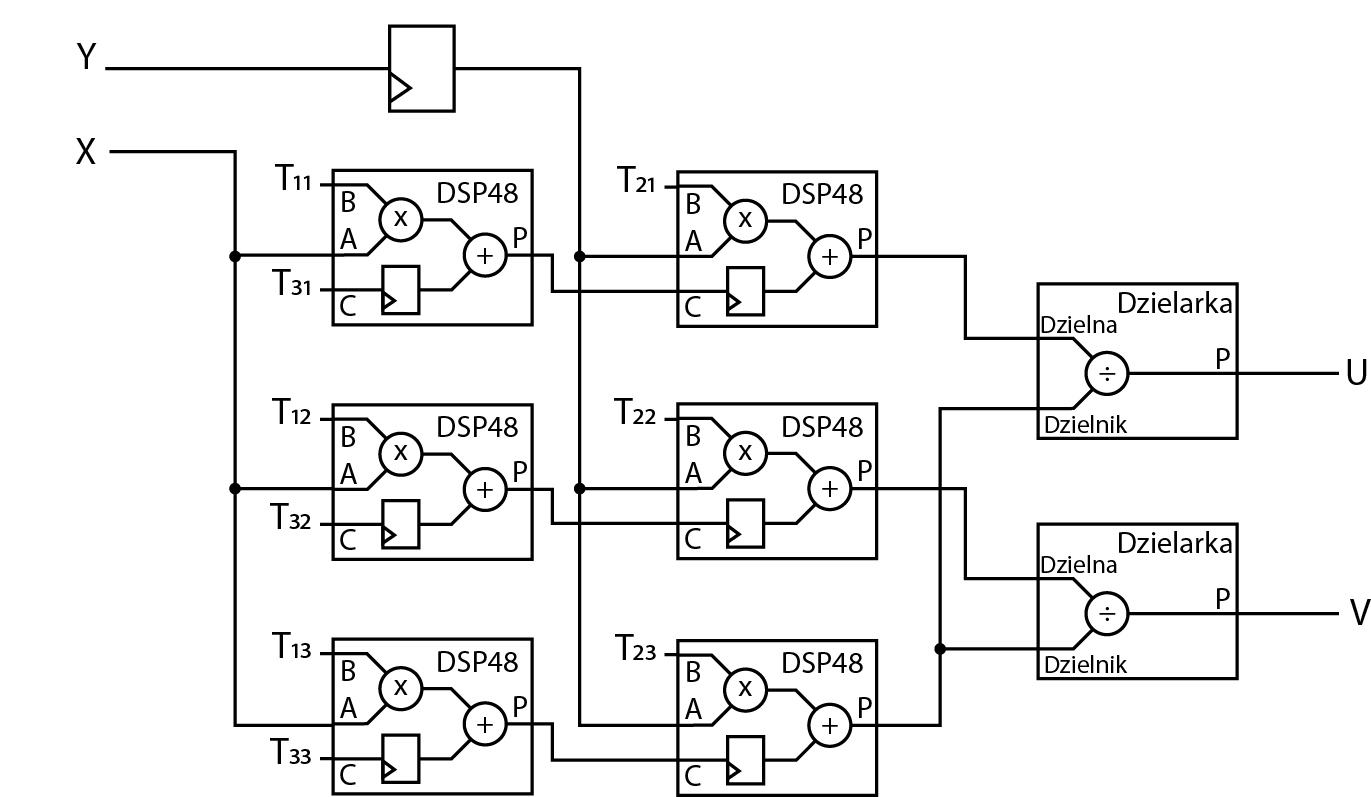
\includegraphics[width=0.70\linewidth]{images/transfProjek.png}
\caption[Schemat modułu transformacji projekcyjnej.]{Schemat modułu transformacji projekcyjnej.}
\label{fig:transfProjek}
\end{figure}

\subsection{Interpolacja dwuliniowa} 
%% Ma za zadanie pobrać z pamięci dwuportowej obrazu IR wartość piksela wskazaną na wejściu układu i wystawić na wyjście. %TODO OK??? a coś jeszzce zrobić -- bo to jest kontorler....
Moduł pozwala na interpolację wartości piksela wskazanego przez koordynaty na wejściu.
Podobnie jak reszta systemu używa AXI4-Stream do przekazywania danych między poszczególnymi modułami.
Dane na wejściu to współrzędne U i~V oraz ich części ułamkowe U\_fraction ($U_f$) i~V\_fraction ($V_f$).
Moduł został wyposażony w~4 rejestry, w~których przechowywane są współrzędne oraz wartości 4 ostatnio użytych pikseli.
Zabieg ten znacznie redukuje liczbę potrzebnych zapytań do pamięci.
Podczas powiększania obrazów istnieje duża szansa, że kolejne koordynaty na wejściu U, V odwołają się do tych samych czterech otaczających ich pikseli (np. [0,0], [1,0], [2,0], podczas zwiększania 10-krotnego, wynikiem transformacji byłyby punkty: [0,0], [0.1,0], [0.2,0], ... więc w~celu interpolacji odwoływałyby się do wartości otaczających ich pikseli: [0,0] , [1,0], [0,1], [1,1]).
W~module następuje sprawdzenie, czy w~pamięci są już wartości z~koordynatów [U, V], [U+1, V] [U, V+1], [U+1, V+1].
Jeżeli któregoś piksela brakuje, jest on pobierany z pamięci i~zapisywany w rejestrze przechowującym niepotrzebny piksel.
Jeżeli wszystkie koordynaty się zgadzają, obliczana jest wartość piksela wyjściowego zgodnie ze wzorem \eqref{equ:bilinear}.

\begin{equation}\label{equ:bilinear}
Ir = A(1-U_{f})(1-V_{f})+B(1-V_{f})+C(1- U_{f})V_{f}+ D U_{f} V_{f}
\end{equation}
\noindent gdzie: $ A, B, C,D $ odpowiadają wartościom pikseli w [U, V], [U+1, V] [U, V+1], [U+1, V+1], a $ Ir $ to wartość wyjściowa piksela wyjściowego.

Moduł działa potokowo. 
W~przypadku gdy wymagana jest  aktualizacja rejestrów, strumień jest wstrzymywany na czas pobrania stosownych wartości z~bufora ramki IR.
Jeżeli koordynaty wejściowe wychodzą poza zakres obrazu termowizyjnego, to ich wartość wyjściowa odgórnie wynosi zero.

\subsection{Łączenie strumieni}

Moduł posiada dwa wejścia AXI4-Stream. 
Strumień RGB jest nadrzędny i~do niego jest dołączany strumień IR. Do synchronizacji została wykorzystana możliwość wstrzymania transmisji poprzez linię \textit{tready} w~interfejsie AXI4-Stream.
Piksele z~dołączanego obrazu są odrzucane do momentu pojawienia się sygnału SOF, reprezentowanym przez wysoki stan linii \textit{tuser}.
Następnie, w~momencie pojawienia się sygnału SOF w~strumieniu głównym transmisja zostaje ponownie wznowiona. 
Po przejściu całej ramki strumienie są ponownie synchronizowane.

\subsection{Koloryzacja i nakładanie}

Strumień RGBIR zostaje połączony w~jeden obraz.
Obraz IR zostaje poddany koloryzacji na podstawie wartości zapisanych w~12-bitowym LUT (ang. \textit{Lookup table}). 
Rysunek \ref{fig:jetPalet} przedstawia użytą paletę do wizualizacji temperatury. 
Obrazy nakładają się w proporcjach 50 na 50. 
Jeżeli wartość piksela IR jest równa zero to nie jest on wyświetlany.
Na wyjściu jest podany 24-bitowy strumień RGB. 
Przykładowy wynik operacji przedstawiono na rysunku \ref{fig:koloryzacja}.
\begin{figure}
\centering
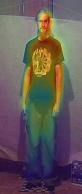
\includegraphics[width=0.3\linewidth]{images/koloryzacja.jpg}
\caption[Obraz IR po koloryzacji i nakłądaniu.]{Obraz IR po koloryzacji i nakładaniu.}
\label{fig:koloryzacja}
\end{figure}

\begin{figure}
\centering
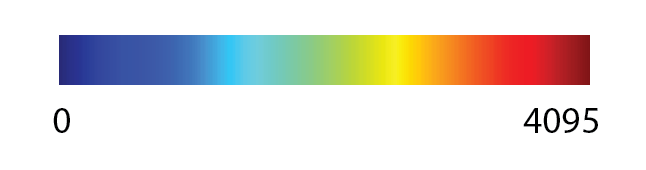
\includegraphics[width=0.5\linewidth]{images/jetPalet.png}
\caption[Paleta kolorów użyta do wizualizacji temperatury.]{Paleta kolorów użyta do wizualizacji temperatury.}
\label{fig:jetPalet}
\end{figure}

\subsection{Obramowanie wyników}

Moduł ma na celu wskazanie na obrazie lokalizacji wykrytego przechodnia, poprzez obramowanie tego obszaru ramką określonego koloru. Kolor, rozmiar i~lokalizacja ramki jest zapisana w dwóch 32-bitowych rejestrach, konfigurowalnych poprzez interfejs AXI4-Lite.

\subsection{Moduł DPM}

Moduł został zaczerpnięty z pracy inżynierskiej autora w~celu selekcji kandydatów w~obrazie multispektralnym i~jest opisany w rozdziale \ref {sec:xiao_2015}. 
Do detekcji wykorzystuje bezpośredni strumień pikseli kamery termowizyjnej. 
Pomocniczy moduł \textit{data grabber} znajdujący się tuż za kontrolerem kamery IR ma za zadanie rozdzielenie sygnału do dwóch komponentów: bufora ramki oraz, po zbinaryzowaniu, do modułu DPM wraz z~jego koordynatami. 
Moduł składa się z~okna kontekstowego o~wymiarach 16x40 pikseli, gdzie odbywa się porównanie z macierzą wzorcową. 
Do każdego piksela w~oknie przypisywana jest wartość ze wzorca LPBW -- jeżeli piksel jest biały albo LPMB w~przypadku czarnego. 
Następnie, wszystkie wartości są sumowane za pomocą drzewa sumacyjnego. Wynikiem jest wartość wyjściowa LP (ang. \textit{Logarithmic Probability}). 
Jeżeli przekroczy ona wartość progową (ustaloną na podstawie sumy LP policzoną dla tła i~parametru K) zostaje przesłana do listy kandydatów wraz ze współrzędnymi tego okna (w~układzie odniesienia kamery IR).
Lista kandydatów jest na bieżąco przesyłana za pomocą AXI4-Stream do pamięci systemu procesorowego poprzez AXI DMA. 
Po sprawdzeniu ostatniego okna zostaje przesłany sygnał \textit{tlast} i~moduł AXI DMA wygeneruje przerwanie w~systemie procesorowym. 
Wartość progowa binaryzacji i~LP jest konfigurowalna za pomocą AXI4-Lite.

\section{System procesorowy}

Program działający w~części procesorowej układu Zynq spełnia dwa podstawowe zadania. 
Po pierwsze pozwala na konfigurację modułów znajdujących się w~PL za pomocą AXI4-Lite. 
Użytkownik za pośrednictwem konsoli może wprowadzać własne parametry dla każdego z modułów. 
Program pozawala również na zapis na karcie SD pojedynczej klatki obrazu multispektralnego, następnego wykrytego ROI oraz ROI znajdującego się pośrodku sceny. 
Ta opcja ułatwiła tworzenie bazy do nauczenia klasyfikatora SVM.

Drugim zadaniem jest klasyfikacja wytypowanego przez DPM kandydata. 
Po otrzymaniu przerwania przez moduł AXI DMA powiązany z DPM, sprawdzana jest lista kandydatów i wybierany jest ten o~największej wartości LP. 
Współrzędne kandydata są podane w~układzie odniesienia kamery IR. 
Po przeliczaniu ich za pomocą macierzy transformacji projekcyjnej i~dodaniu pewnego \textit{offsetu} w~buforze ramki obrazu RGBIR zostaje wskazane ROI o~wymiarach 80x192 pikseli. 
Następnie, obliczany jest wektor cech HOG z~tego obszaru. 
Potem na jego podstawie odbywa się klasyfikacja przy użyciu wytrenowanego SVM. 
Wynik klasyfikacji jest wyświetlany w~konsoli wraz z~jego współrzędnymi na obrazie i~wartością LP. 
Dodatkowo obszar ten zostanie zaznaczony zieloną ramką na wyjściowym strumieniu wizyjnym. 
Jeżeli kandydat nie zostanie zakwalifikowany pozytywnie przez SVM ramka przybierze kolor czerwony. 
Brak kandydatów wskazuje czarna ramka w~miejscu ostatniej detekcji.

\section{Proces kalibracji}
W~celu kalibracji, zostaje wykonane zdjęcie specjalnej planszy kalibracyjnej za pomocą obu kamer (rysunki \ref{fig:calibrationThermal}, \ref{fig:calibrationRGB}). 
%TODO 2 a co to ,,świeci'' na tej planszy...
Pozwala to na identyfikację czterech punktów kalibracyjnych w~obu przestrzeniach: RGB i~IR. 
Następnie na ich podstawie zostaje obliczona macierz transformacji projekcyjnej. 
Na rysunku \ref{fig:calibrationCorrectedGrey} przedstawiono obraz z~kamery termowizyjnej po transformacji, który pokrywa się z obrazem wizyjnym (rysunek \ref{fig:calibrationSum}).

\begin{figure}[h]
\centering
\begin{subfigure}{0.47\textwidth}
\centering
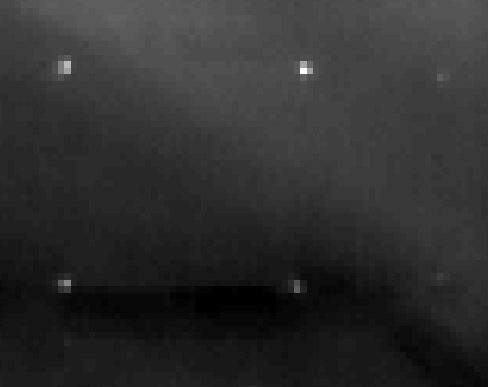
\includegraphics[width=0.9\linewidth]{images/calibrationThermal}
\subcaption{\label{fig:calibrationThermal}}
\end{subfigure}
\begin{subfigure}{0.47\textwidth}
\centering
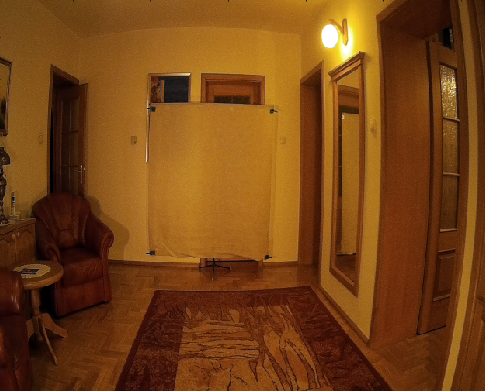
\includegraphics[width=0.9\linewidth]{images/calibrationRGB}
\subcaption{\label{fig:calibrationRGB}}
\end{subfigure}
\begin{subfigure}{0.47\textwidth}
\centering
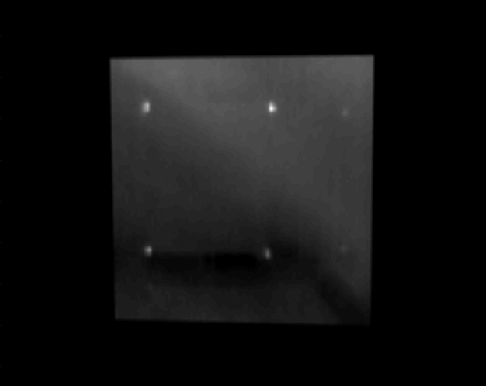
\includegraphics[width=0.9\linewidth]{images/calibrationCorrectedGrey}
\subcaption{\label{fig:calibrationCorrectedGrey}}
\end{subfigure}
\begin{subfigure}{0.47\textwidth}
\centering
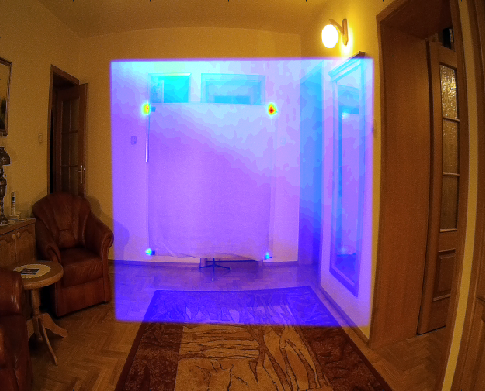
\includegraphics[width=0.9\linewidth]{images/calibrationSum}
\subcaption{\label{fig:calibrationSum}}
\end{subfigure}
\caption[Proces kalibracji]{Proces kalibracji: \protect\subref{fig:calibrationThermal} obraz z kamery termowizyjnej, \protect\subref{fig:calibrationRGB} obraz z kamery wizyjnej, \protect
\subref{fig:calibrationCorrectedGrey} obraz z kamery termowizyjnej po transformacji projekcyjnej, \protect\subref{fig:calibrationSum} obraz z kamery termowizyjnej po transformacji projekcyjnej nałożony na obraz z kamery wiyjnej.}
\end{figure}

\section{HOG i SVM}
%TODO 2 coś nie halo 1. Gradienty. 2. Potem podział.
Okno detekcji zostaje podzielone na 60 komórek o wielkości 16x16 pikseli. %TODO 2 jakieś zdanie wprowadzenia ?
Następnie obliczane są gradienty dla poszczególnych pikseli. 

Pojedynczy gradient składa się z kierunku oraz wartości wypadkowej.
%TODO Gradient dla pojedynczego piskela ma amplitude (moduł) i kierunek.

%TODO Teraz podział i obliczanie histogramu w komórkach

Wykorzystany jest histogram ważony o 9 przedziałach. 
Oznacza to, że wartość wypadkowa gradientu jest dzielona na dwa przedziały, pomiędzy którymi się znajduje w proporcjach określonych wzorem \eqref{equ:bin1}, \eqref{equ:bin2}.
%TODO wypadkowa -> moduł !!
\begin{equation}\label{equ:bin0}
Bin1_{dir} < G_{dir} < Bin2_{dir}
\end{equation}
\begin{equation}\label{equ:bin1}
Bin1_{mag} = \frac{Bin2_{dir} - G_{dir}}{Bin2_{dir} - Bin1_{dir}}
\end{equation}
\begin{equation}\label{equ:bin2}
Bin2_{mag} = \frac{G_{dir}- Bin1_{dri}}{Bin2_{dir} - Bin1_{dir}}
\end{equation}
\noindent gdzie: $G_{dir}$ to kierunek badanego gradient, $G_{mag}$ to wypadkowa badanego gradientu, $Bin1_{dir}$,$Bin2_{dir}$ to kierunki gradientów powiązane z danym przedziałem histogramu, $Bin1_{mag}$,$Bin2_{mag}$ to wypadkowa gradientu przypisana do poszczególnego z przedziału.
%TODO wypadkowe.... 

Dla każdej z komórek dodatkowo obliczana jest suma kwadratów wartości przedziałów histogramu.
Następnie komórki są łączone w~bloki 2 na 2, w~których obrębie dokonywana jest normalizacja, wykorzystując wcześniej obliczone sumy kwadratów. 
Zastosowano normalizację L2 wyrażoną wzorem \eqref{eq:norm}.
\begin{equation}\label{eq:norm}
norm = \sqrt{\sum_{i} (Bin(i)_{mag})^2 + c}
\end{equation}
\noindent gdzie: $Bin(i)_{mag}$ to wartość przedziału histogramu, a $c$ to mała wartość stała.
Następnie wartości wszystkich 36 przedziałów w~4 histogramach są dzielone przez $norm$.
Bloki nakładają się na siebie, zatem w~pojedynczym oknie można wyodrębnić 44 bloki. 
Suma histogramów z~wszystkich bloków tworzy 1584-elementowy wektor cech.

W~celu wytrenowania klasyfikatora SVM zostało wykonane 60 obrazów -- 30 pozytywnych zawierających przechodnia i~30 przedstawiają elementy tła lub niekompletnej sylwetki człowieka (np. sama ręka).
Jest to klasyfikator liniowy. %TODO 2 a to zdanie do czego... nie pasuje kompletnie... i nieco szerszy opis SVM.
Do każdej z cech jest przypisana jej waga. 
Po zsumowaniu wszystkich wag dodawany jest $bias$. %TODO iloczyn wagi i cechy jak już.
Jeżeli wynik jest większy od zera świadczy to o~pozytywnym wyniku klasyfikacji.

\section{Wyniki}

Aby sprawdzić działanie i~dokładność systemu została zaimplementowana możliwość zapisu obliczonego wektora cech na karcie SD.
Następnie został obliczony przykładowy błąd względny między wektorem cech wyliczonym w pakiecie Matlab, a uzyskanym z systemu wizyjnego. %TODO 2 powt. obliczony i dlaczego przykładowy ?
Błąd oscyluje w~granicy \(10^{-6}\) co czyni go marginalnym i~najprawdopodobniej wynika z~różnic w użytych bibliotekach numerycznych. 
Świadczy to o prawidłowym działaniu systemu.

Na przebadanie jednego okna zaproponowany system potrzebuje 75 ms (dla porównania te same obliczenia w~pakiecie Matlab zajmują około 23 ms przy użyciu komputera z procesorem Pentium Core i7 i~8GB pamięci RAM).
Dzięki zastosowaniu sprzętowego wyszukiwania ROI zadanie systemu procesorowego zostało ograniczone do analizy pojedynczego ROI. 
Kamera termowizyjna, będąca źródłem sygnału dla wzorca probabilistycznego, pracuje z prędkością 9 klatek na sekundę co zapewnia 111 ms na analizę jednej rami obrazu. 
Ponieważ analiza jednego okna zajmuje 75 ms  możliwe sprawdzenie tylko jednego ROI na ramkę. 
Na rysunku \ref{fig:workingSystem} przedstawiono zdjęcie działającego systemu.

\begin{figure}
\centering
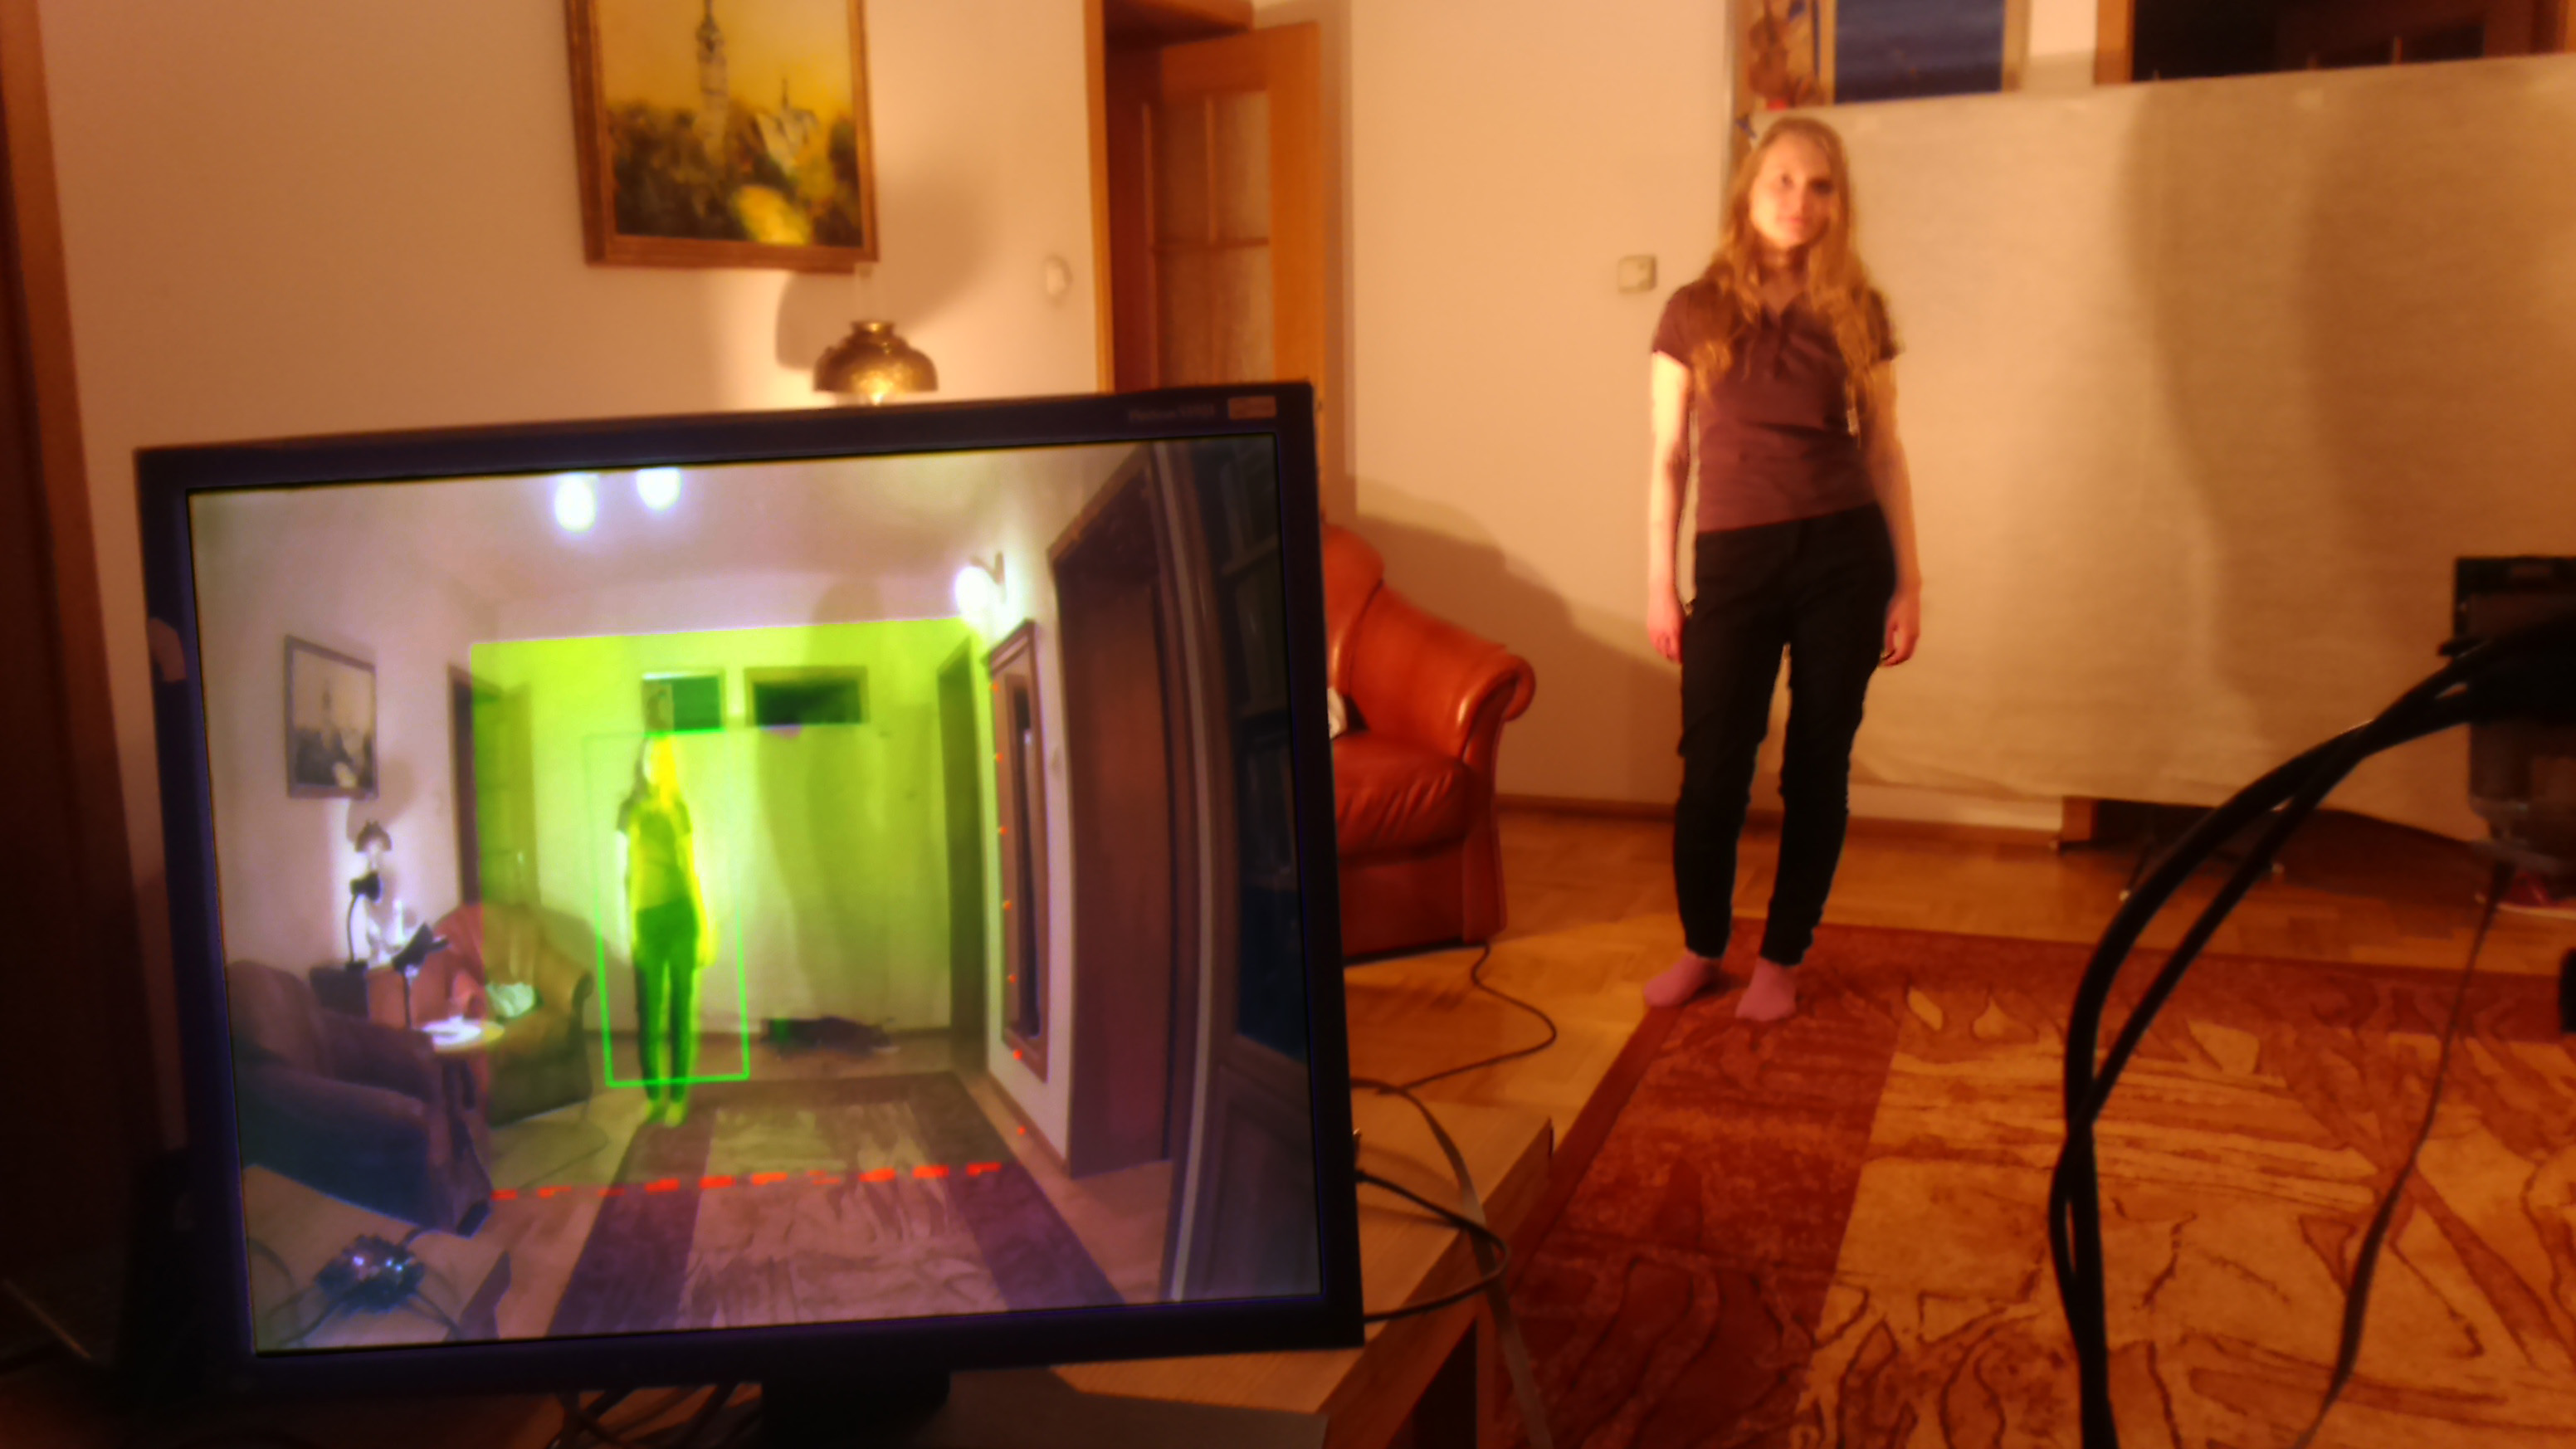
\includegraphics[width=0.8\linewidth]{images/workingSystem.jpg}
\caption[Działający system.]{Działający system.}
\label{fig:workingSystem}
\end{figure}

%TODO no ale jakby to dla 30/60 fps... to już tak pięknie nie jest %% TT Mam w zapasie moduł który liczy gradienty oraz przedział i histogram pojedynczego piksela, tylko dodanie go powoduje że układ jest niesyntezowalny
%TODO 2 to to w future work...
W~tabeli \ref{tab:fpgautilization} zostało przedstawione wykorzystanie zasobów logiki programowalnej.
\begin{table}[]
\centering
\caption{Wykorzystane zasoby logiki programowalnej.}
\label{tab:fpgautilization}
\begin{tabular}{|l|l|l|l|}
\hline
Element & Wykorzystane & Dostępne & \% \\ \hline 
LUT & 12583 & 17600 & 71,49 \\ \hline
LUTRAM & 617 & 6000 & 10,28 \\ \hline
FF & 19924 & 35200 & 56,60 \\ \hline
BRAM & 25,50 & 60 & 42,50 \\ \hline
DSP & 36 & 80 & 45,00 \\ \hline
IO & 43 & 100 & 43,00 \\ \hline
BUFG & 7 & 32 & 21,88 \\ \hline
MMCM & 1 & 2 & 50,00 \\ \hline
PLL & 1 & 2 & 50,00 \\ \hline
\end{tabular}
\end{table}

%TODO 2 Tu mogłby Pan kilka zdań komentarza do tabelki. Co jest przyczyną takiego, a nie innego wykorzystania.

\chapter{Podsumowanie i możliwe dalsze kierunki rozwoju systemu}

Zgodnie z celem pracy został opracowany system detekcji przechodniów na podstawie obrazu z kamery termowizyjnej. 
Mając do dyspozycji kamerę Lepton o~bardzo małej rozdzielczości (80x60 pikseli) zdecydowano się na wykorzystanie obrazu wizyjnego i detekcję obiektów w przestrzeni multispektralnej (RGBIR). 
W~tym celu, zgodnie z założeniem, wykorzystano heterogeniczny układ Zynq-7000 umożliwiający sprzętowo-programową implementację algorytmów.
Zadaniem części logiki programowalnej (FPGA) było połączenie strumieni wizyjnych z~kamer w~jeden obraz multispektralny oraz określenie obszaru zainteresowania (ROI) do klasyfikacji. 
W celu określenia ROI został wykorzystany słabszy klasyfikator: wzorzec probabilistyczny -- opracowany przez autora w~ramach pracy inżynierskiej. 
Wytypowany kandydat był następnie klasyfikowany przy użyciu deskryptora HOG i~SVM. 
Proces ten odbywał się w~systemie procesorowym układu Zynq. 
Drugim zadaniem systemu procesorowego była konfiguracja parametrów modułów zaimplementowanych w~logice programowalnej oraz wizualizacja wyników. 
Dodatkowa funkcja zapisania obrazów na karcie SD dała możliwość stworzenia własnej bazy próbek do nauczenia klasyfikatora.

Zastosowana kamera termowizyjna umożliwia akwizycję 9 klatek na sekundę i~jest źródłem obrazu dla modułu odpowiedzialnego za określanie ROI. 
Ponieważ system procesorowy potrzebuje 75 ms na klasyfikację pojedynczego ROI, a~kolejne ramki obrazu pojawiają się co około 111 ms możliwa jest tylko jedna detekcja na klatkę obrazu IR. 
Nie jest to imponujący wynik. %OK TODO słabszy to złe słowo, poza tym... co to są inne.

W~celu poprawy szybkości działania można by przenieść obliczanie deskryptora HOG związaną z~systemu procesorowego do logiki programowalnej, ale nie pozwalają na to ograniczone zasoby logiczne używanego układu Zynq. 
Na podstawie modelu programowego można stwierdzić, że w porównaniu do poprzedniego systemu spadła liczba fałszywych pozytywnych detekcji. 

Dalszym kierunkiem rozwoju byłoby dodanie drugiej kamery termowizyjnej Lepton, co pozwoliłoby na otrzymanie obrazu stereoskopowego, by estymować odległość od obiektu. Mając tę informację można automatycznie dopasowywać wielkość wzorca odpowiadającą sylwetce przechodnia w danej odległości od kamery. Mała rozdzielczość czujnika również zachęca do analizy ruchu. Poprzednią ramkę obrazu można przechować bezpośrednio w pamięci BRAM układu FPGA i wykorzystać do strumieniowego obliczania lokalnego przepływu optycznego. Na jego podstawie system wspomagania kierowcy mógłby wykryć czy wykryty przechodzień może wtargnąć przed pojazd.
%TODO 2 1. Raczej, że fuzja danych czy coś.
%OK TODO 2. Proszę już coś wymyleć inna kamera, analiza ruchu, śledzenie, itp. No na pewno ma Pan jakieś pomysły.
\nocite{*}
\printbibliography
\appendix
\chapter{Dodatek A -- zawartość płyty CD}
\begin{itemize}
\item /doc -- tekst pracy dyplomowej,
\item /src -- użyte skrypty i funkcje napisane w języku Matlab,
\item /bootimage -- plik rozruchowy dla platformy Zybo,
\item /vivado -- projekt w programie Vivado.
\end{itemize}
%OK TODO A projekt Vivado ?









\chapter{Dodatek B -- Instrukcja obsługi systemu}

%TODO A tu nie trzeba jeszcze włożyć karty SD ? Bo rozumiem, że to tak startuje
%TODO Jeszcz taki informtyczny opis projektu - co jest w jakim pliku.

Aplikacja uruchamia sie z karty SD. Po podpięciu platformy Zybo przez złącze mikro USB uzyskujemy dostęp do terminalu poprzez UART. 
Parametry portu: baud rate 115200, 8 bitów, jeden bit stopu, brak kontroli parzystości.

Wciśnięcie klawisza 'h' powoduje pokazania się karty pomocy:

\begin{lstlisting}
HELP:
1 VDMA status
2 Start detection
3 Restart DMA

5 read T matrix
6 write T matrix
7 write bin threshold
8 update LP threshold

w save next detected ROI
s save centered ROI
x save center ROI and HOG discriptor
d save whole frame
m mount SD card
q get calibration image

\end{lstlisting}
 
\noindent Wprowadzenie znaku z~powyższej listy do konsoli powoduje wykonanie następującej akcji:
 
\begin{itemize}
\item 1 -- wyświetlenie statusu VDMA,
\item 2 -- rozpoczęcie detekcji przechodniów,
\item 3 -- restart DMA,
\item 5 -- wyświetlenie parametrów macierzy transformacji projekcyjnej,
\item 6 -- pozwala na wprowadzenie nowej macierzy T. Dane należy wprowadzić w postaci 9 liczb z przecinkiem (kropką) np.: wprowadzenie ''1.0 0.0 0.0 0.0 1.0 0.0 0.0 0.0 1.0'' zamienia macierz T na macierz jednostkową,
\item 7 -- pozwala na wprowadzenie progu binaryzacji dla modułu DPM,
\item 8 -- pozwala na wprowadzenie progu LP dla modułu DPM,
\item w -- zapisanie następnego wykrytego ROI w~postaci pliku ROInnn.CIR gdze nnn to kolejne numery plików.
\item s -- zapisanie ROI znajdującego się na środku obrazu w~postaci pliku ROInnn.CIR gdzie nnn to kolejne numery plików.
\item x -- zapisanie ROI znajdującego się na środku obrazu w~postaci pliku ROInnn.CIR  oraz wektora cech w postaci pliku FVnnn.FLO nnn to kolejne numery plików.
\item d -- zapisanie całej ramki obrazu w~postaci pliku FRAMEnnn.CIR gdzie nnn to kolejne numery plików.
\item m -- zamontowanie karty SD w celu zapisu plików,
\item q -- zapis obrazu kalibracyjnego w~postaci pliku CALIBR.CIR. Spowoduje to zapisanie obrazu wizyjnego wraz z~niepoddanym transformacji obrazem termowizyjnym.
\end{itemize}

Pliki .CIR można otworzyć za pomocą funkcji [IrImage, rgbImage] = cir2image( filename ) w pakiecie MatLab (znjdującym się na płycie CD w folderze /src). Zwraca ona dwie macierze: IrImage -- zapisany obraz w podczerwieni oraz rgbImage zapisany obraz wizyjny.

Pliki .FLO składa się z 1584 32-bitowych liczb zmiennoprzecinkowych typu float. 
Reprezentuje on obliczony przez procesor wektor cech związanego z nim ROI.





\end{document}
